\chapter{Materials and Methods}

In this section, we describe the steps required to get from a primary protein sequence to its tertiary structure.
It begins with the description of the input. 
The second part focuses on the model choices and mainly describes the convolutional neural network. 
The last section focuses on structure realization. 
A graphical overview of the entire pipeline is shown in Figure \ref{fig:project_pipeline}. 
%In each of the 3 subsections, the corresponding part of the diagram will be unravelled to accompany the verbal descriptions.

\begin{figure}[ht]
    \centering
    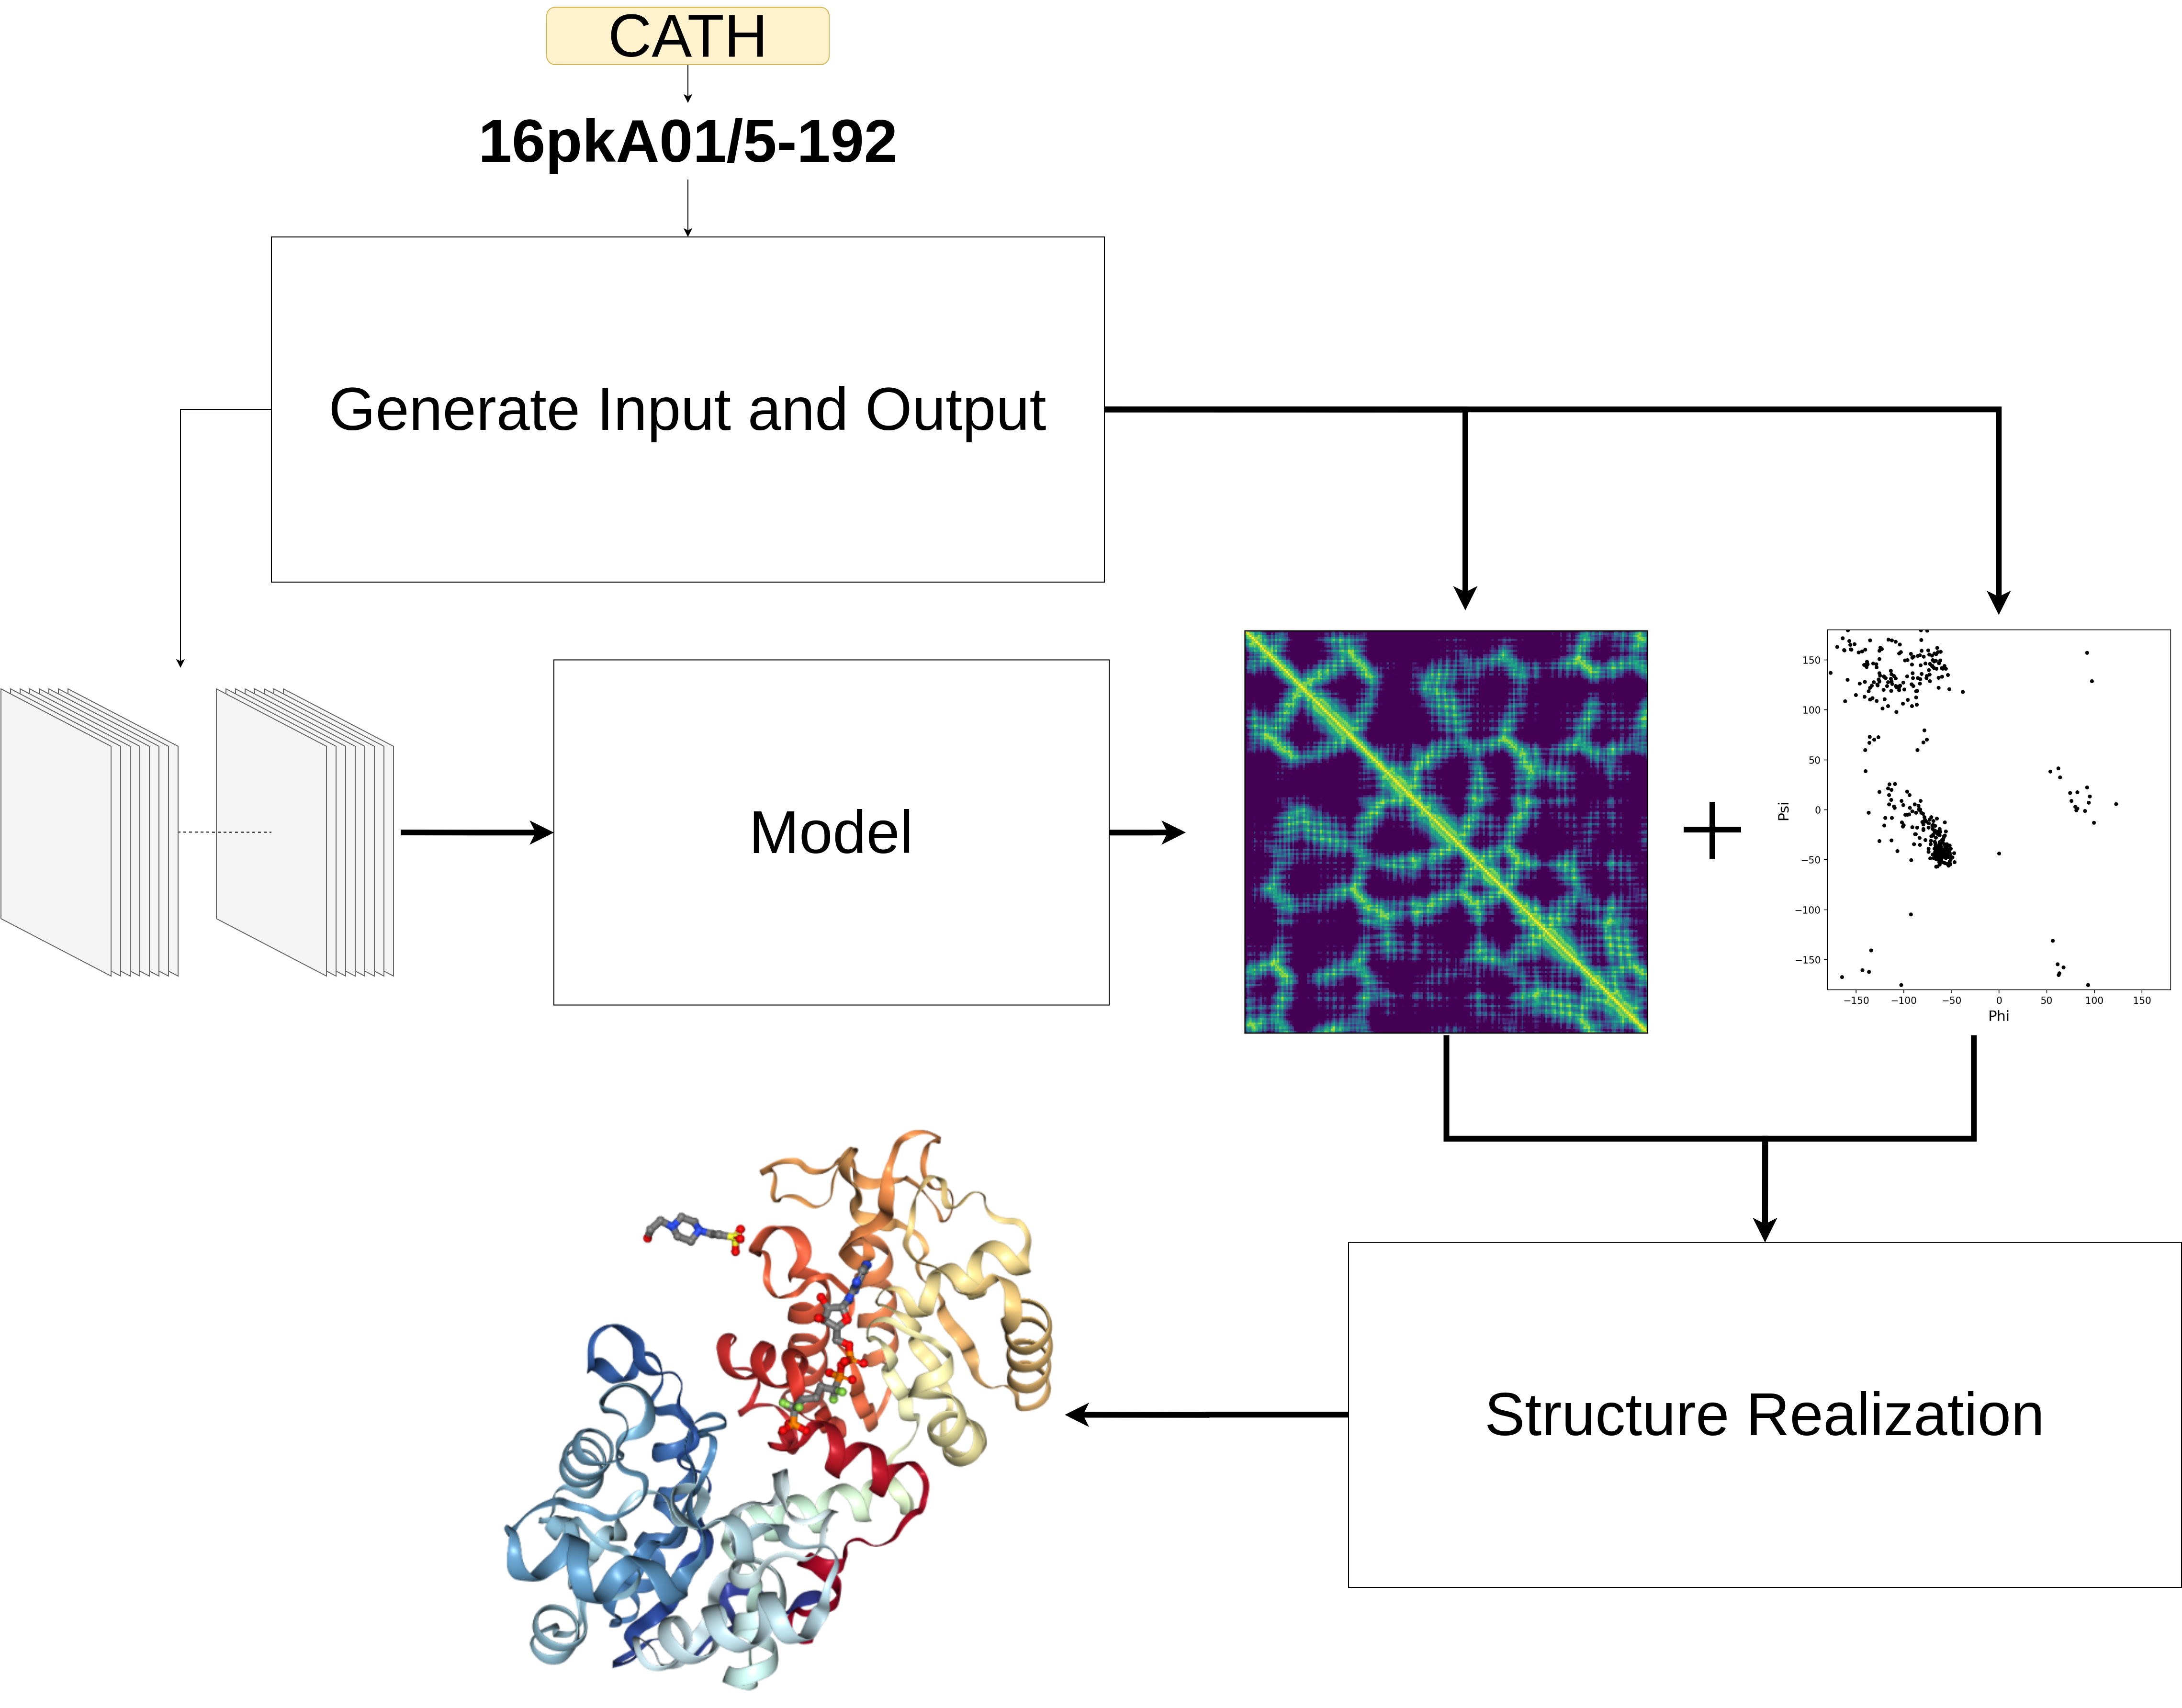
\includegraphics[width=\linewidth]{imgs_tomas/Project_pipeline_small.png}
    \caption{Pipeline overview}
    \label{fig:project_pipeline}
\end{figure}

\section{Primary Sequence to CNN Input}

% \begin{figure}
%     \centering
%     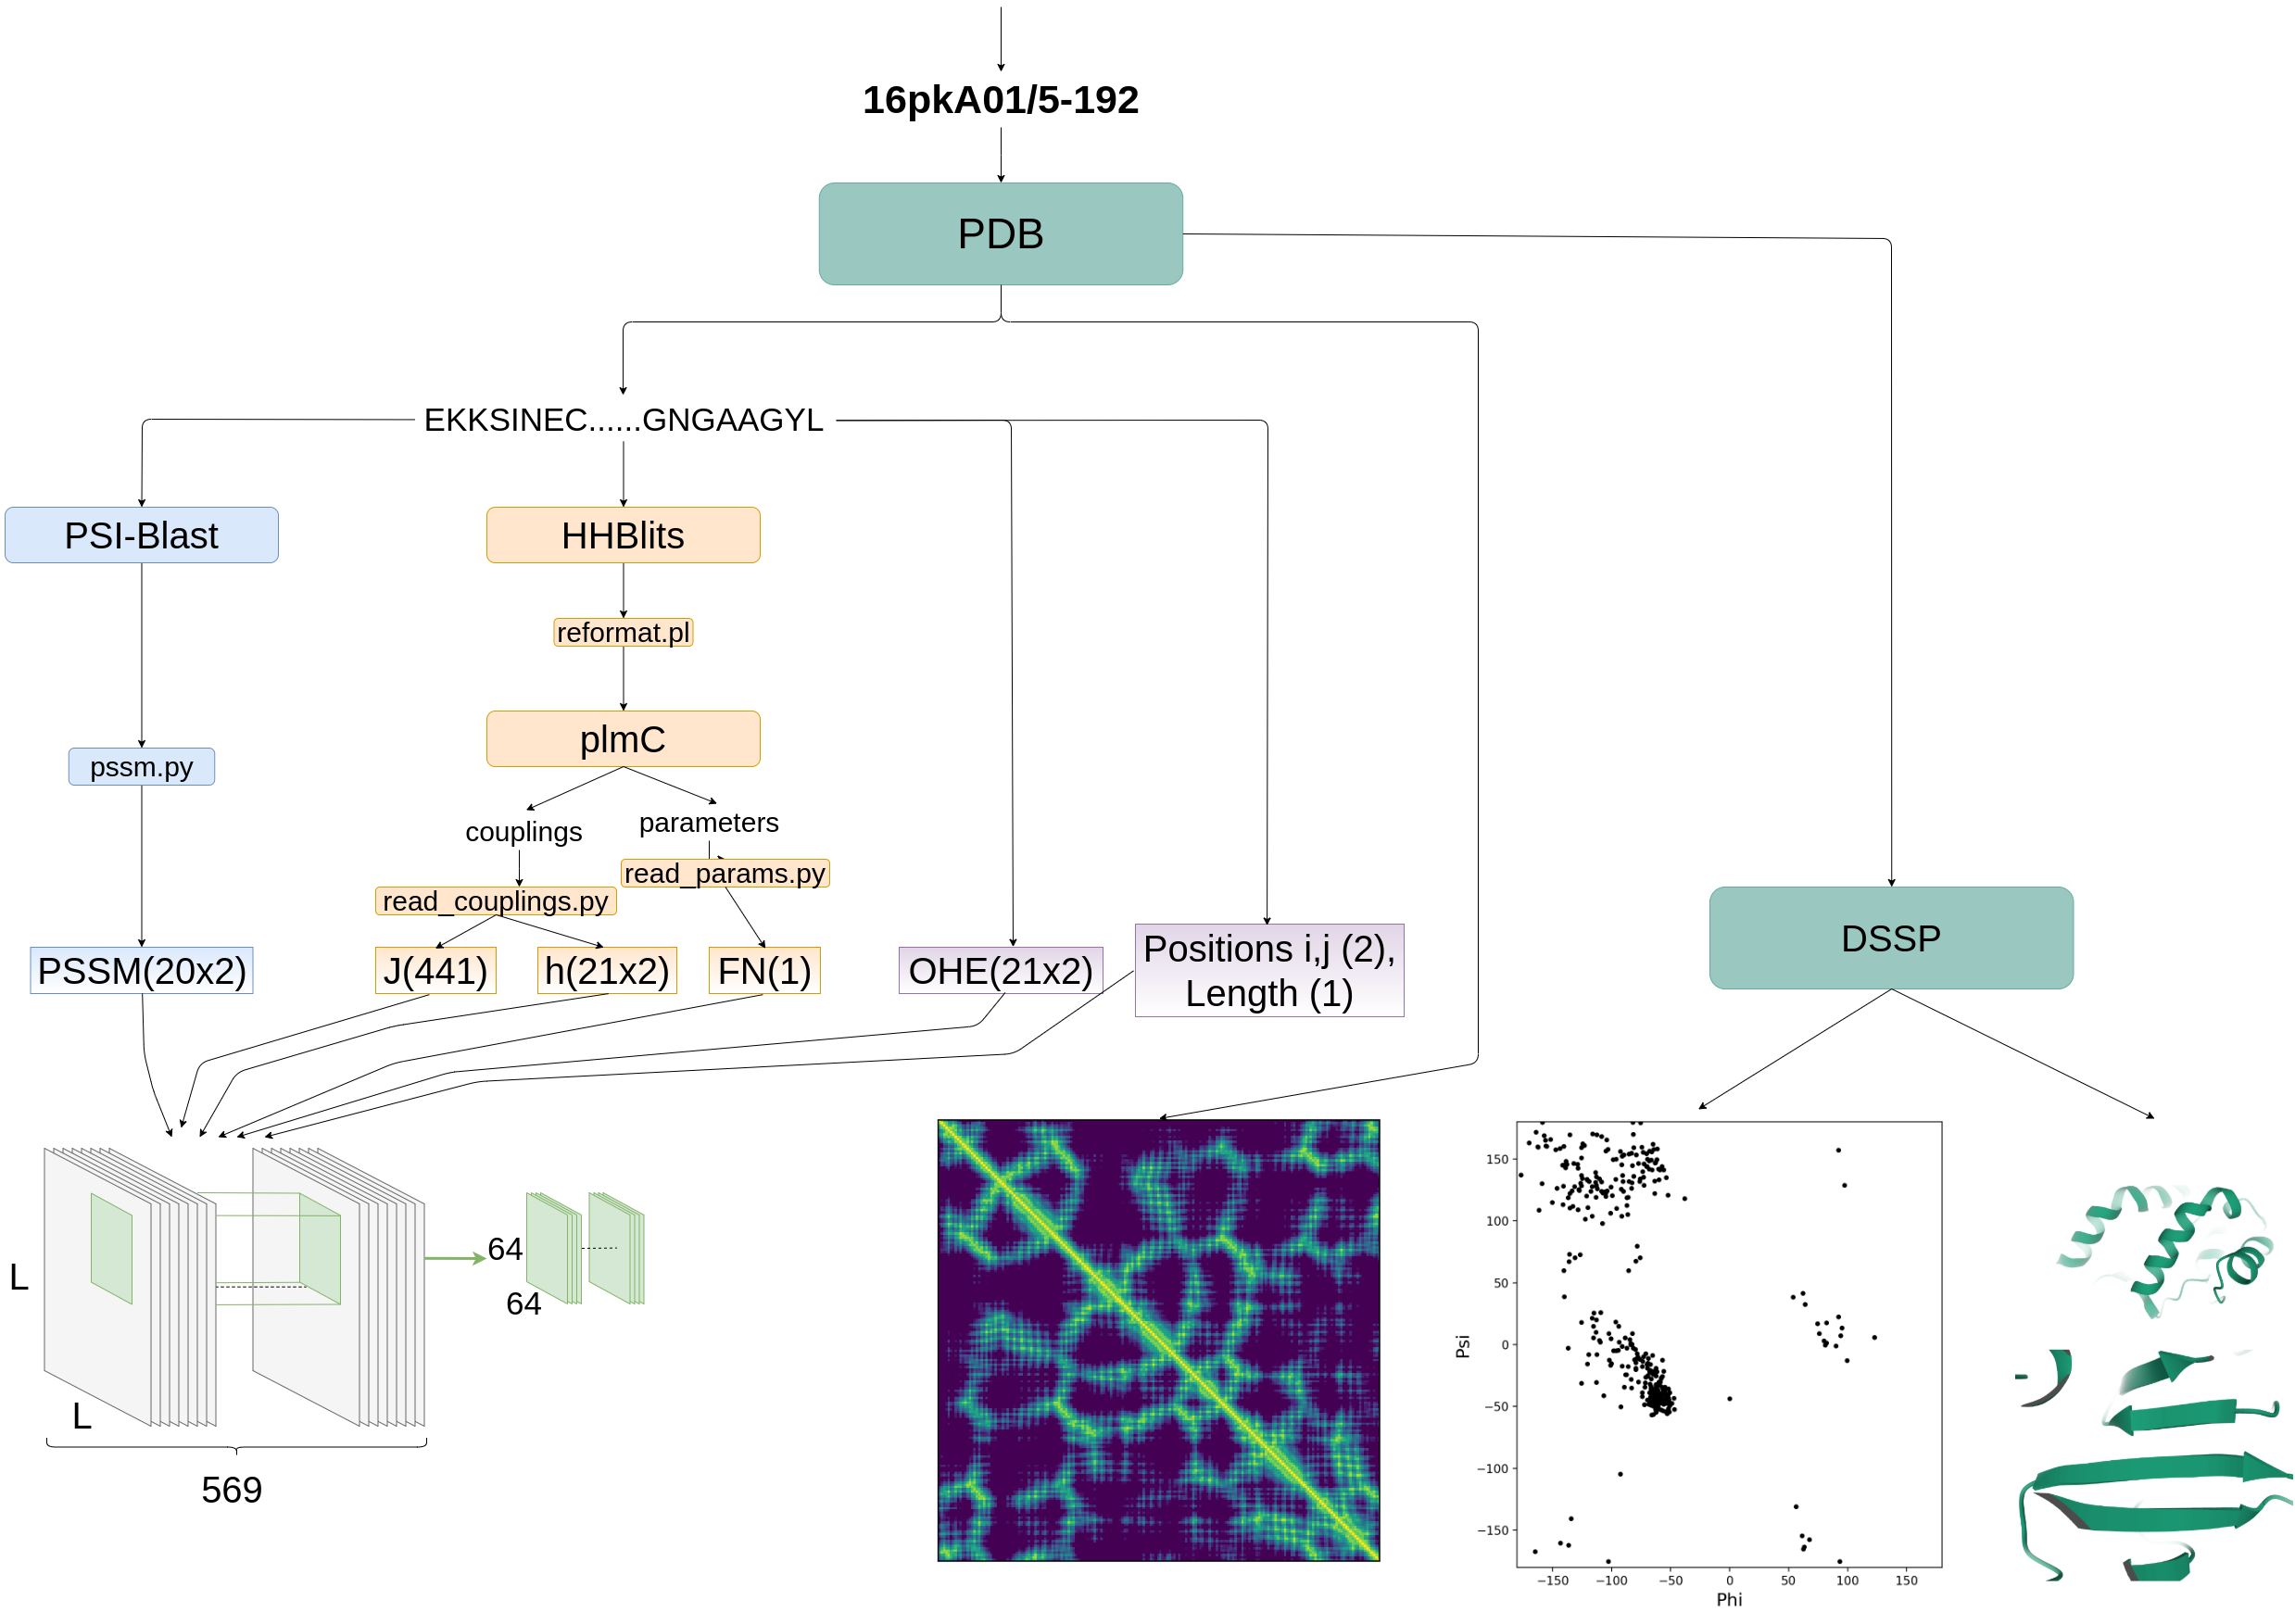
\includegraphics[width=\linewidth]{imgs_tomas/pipeline_input.png}
%     \caption{Input / Output data generation}
%     \label{fig:pipeline_input}
% \end{figure}

The primary sequence of proteins is usually recorded in the FASTA format.
This is one of the most commonly used formats in bioinformatics.
It is typically stored as a plain text file, possibly compressed. 
Each record in FASTA format consists of a description line, starting with $>$ character, followed by a unique identifier of the particular sequence and a sequence.
The sequence starts on a new line and is represented by single-letter codes.
It is common to split very long sequences to multiple lines.
One FASTA file can contain many records.
An example of this format is shown in the Figure \ref{fig:fasta}.

\begin{figure}[ht]
    \centering
    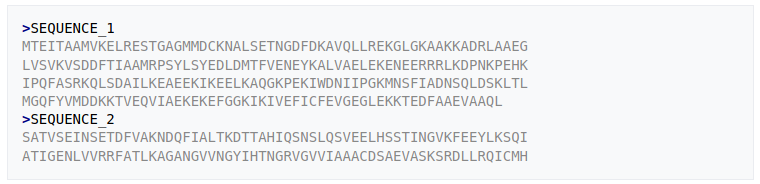
\includegraphics[width=\linewidth]{imgs_andy/fasta.png}
    \caption{Example of protein sequences in FASTA format.}
    \label{fig:fasta}
\end{figure}

In our project, we used the FASTA format as the only input format to our pipeline.
All other characteristics of the protein were calculated from this format.

\subsection{Sequence search and MSA construction}

During evolution, we expect that functional parts of proteins are going to be conserved. 
Furthermore, we expect that two amino acids that are close to each other in the 3D space (not necessarily in the primary sequence) are going to co-evolve as well. 
This co-evolution of spatially proximal amino acids should be reflected in the Multiple Sequence Alignment (MSA) of related proteins.

To formalize the notion of relatedness of the proteins, we can use the edit distance of the sequences.
The edit distance is the minimal number of operations, such as insertions, deletions or substitutions, required to transform one sequence of letters to another.
The best possible distance score in these settings is 0 and is achievable only when we are measuring the distance between identical proteins.
The higher values of the score can then be interpreted as a result of comparing less similar sequences.
In bioinformatics, more complex weighting schemes can be used to reflect the underlying biology, e.g. substitution of one hydrophobic amino acid for another hydrophobic amino acid can be penalized by lower value than the substitution of hydrophobic amino acid for hydrophilic. 

Now, with this definition of relatedness, we could try to compute the distance score for every pair of the proteins considered in the analysis.
Using the dynamic programming, computing the score for one pair takes $\mathcal{O}(m \cdot n)$ time, where $m$ and $n$ are the lengths of the two sequences.
Unfortunately, this approach quickly becomes impractical as the number of sequences considered reach tens of thousands and therefore, we need something more efficient.

A more efficient approach is to use the Basic Local Alignment Search Tool (BLAST) \cite{altschul1990basic}.
It is a heuristic algorithm, based on the short exact word pairs.
At first, the database from all considered sequences is constructed.
Then, we take one sequence, also called the query sequence, and create all k-letter words from it.
These k-letter words are then filtered using a scoring matrix and a parameter $T$ in such a way that only informative words will remain.
The informative words are then mapped to the database using a quick exact search.
This creates hits, which are then extended using dynamic programming.
At the end only hits with alignment score above a certain threshold are kept.

Although BLAST does not guarantee to discover all similar sequences, the results are usually very close to the optimum and the time consumption of this algorithm is much lower.

After the sequence search, we want to create a Multiple Sequence Alignment from the identified similar sequences.
The MSA can be formally defined as a matrix of size $N \times L$ containing 1-letter codes for amino acids or "-" symbolizing a gap, where $N$ is the number of sequences in the alignment and $L$ is the length of the alignment.
Generally, we are interested in the MSA, which minimizes score similar to the distance score used previously.
To find an optimal MSA is an NP-complete problem, but fortunately there exist heuristic approaches, which produce a good MSA in a reasonable time. 

% checkpoint 20200602
\subsection{Position-specific Scoring Matrix}

Position-specific Scoring Matrix (PSSM) is generally used to represent biologically important patterns across multiple sequences. 

To create the PSSM, let's assume that we already constructed a multiple sequence alignment (MSA) of our target sequence and related proteins.
This multiple sequence alignment consists of $N$ rows representing sequences and $L$ columns representing positions of alignment.
Furthermore, each sequence is a sequence of letters from an alphabet with $Q$ symbols.

Then, the first step in the creation of PSSM is the calculation of the Position Frequency Matrix (PFM), by simply counting the number of occurrences of a symbol at a position in the MSA.
Formally, PFM is a matrix with $Q$ rows and $L$ columns, where each entry $\text{PFM}_{q, l}$ is given by Equation \ref{eq:pfm}.

\begin{equation}
    \text{PFM}_{q, l} = \sum_{n = 1}^{N} \delta(\text{MSA}_{n, l}, q)
    \label{eq:pfm}
\end{equation}

From the PFM, a Position Probability Matrix (PPM) is then created simply by scaling the counts by the number of sequences in the MSA.
Therefore:

\begin{equation}
    \text{PPM}_{q, l} = \frac{1}{N} \text{PFM}_{q, l}
\end{equation}

The PSSM is then defined as the log-likelihoods of the PPM transformed by some background model $b$.
For example, the simplest background model might be the one, where each symbol appears in the sequences equally likely, thus $b_q = \frac{1}{Q}$.
This definition gives us the Equation \ref{eq:pssm}.

\begin{equation}
    \text{PSSM}_{q, l} = \log_2 \frac{\text{PPM}_{q, l}}{b_q}
    \label{eq:pssm}
\end{equation}

In practice, more complex background models, such as the total frequency of a symbol in the entire MSA, is often used.
Moreover, it is often encountered, especially when the number of sequences in the MSA is small, that some entries of the PFM are zeroes.
This is an issue because it renders some sequences impossible even though they might be just very unlikely and due to the limited number of samples not observed.
To address this issue, pseudo counts are often used.
This means that we start the PFM construction with one assigned to every entry instead of zero.
It will ensure that the probabilities in the PPM will be non-zero and it also accounts for finite sample size.

\subsection{Potts Models}

\begin{figure}
    \centering
    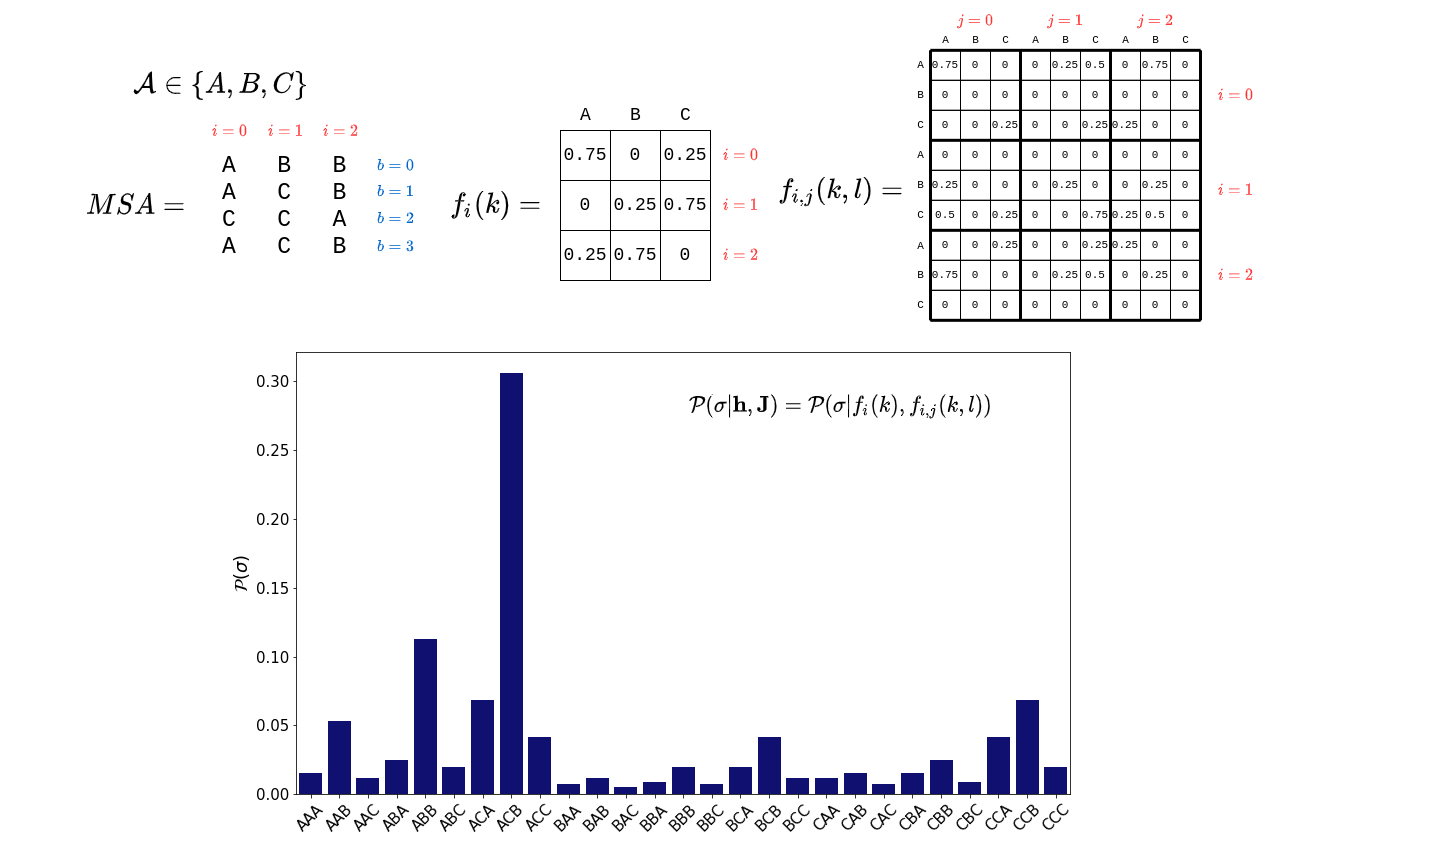
\includegraphics[width=\linewidth]{imgs_tomas/potts_example.png}
    \caption{Potts model example for an MSA shown in the upper left corner and the exact parameters calculated. In the bottom is a plot of probabilities for each unique sequence consisting of 3 symbols, calculated using the potts model formula \ref{eq:Potts}}
    \label{fig:potts_example}
\end{figure}

The Potts model describes a probability distribution derived from a Multiple Sequence Alignment for any sequence of given constant length. The function has only two parameters: one describing the propensities of symbols in MSA (similar to the PSSM) and one describing pairwise interactions of symbols. For very short sequences the Potts model can be calculated exactly. However this is not feasible in practice, which means that one must resort to gradient descent based techniques. 

The most difficult part for finding Potts Model parameters is to ensure that the probabilities for all sequences sum to one. For this one would need to calculate the value of Potts Model function for all sequences of some length composed of symbols from given alphabet. For example for sequence length of 10 and alphabet of size 21 (number of amino acids + gap), there are $10^{21}$ unique sequences.

An example of Potts model for sequence of length 3 composed of symbols from Alphabet \{A, B, C\} is shown on Figure \ref{fig:potts_example}.

Here one can simply calculate the frequencies and connected frequencies of amino acids in the MSA and then calculate the corresponding Potts Model values (described in more detail in next section). The sum of all these values acts as a normalizing constant for the final model (also called a partition function in later description). 

\subsubsection{Potts Models formalized}
Let us assume that we have a sequence $\boldsymbol{\sigma} = (\sigma_1, \sigma_2, ..., \sigma_L)$, where $L$ is the length of the multiple sequence alignment. 
Let us further assume that each symbol $\sigma_i$ in the sequence comes from an alphabet $\mathcal{A} = (a_1, a_2, ..., a_Q)$ of size $Q$. 
Thus for sequence length $L$ we can generate $Q^L$ number of unique sequences.
    
In our case, the sequence $\boldsymbol{\sigma}$ is some sequence of amino acids, and thus the alphabet size is equal $Q = 21$ (20 amino acids, 1 gap symbol).
        
Given a MSA, we would like to find pairs of amino acids that are coupled, i.e. the pairs of amino acids that are correlated due to their direct contact. 
The reason why we can not use correlation data directly is that some pairs of amino acids might be correlated through some intermediate paths.
        
We have to keep in mind that MSA is only generated from a sample of sequences.
Thus it can only help us to estimate the frequencies and connected correlations of amino acids. 
To calculate the connected correlation of a pair of amino acid, we use the covariance Equation \ref{eq:cov}.

\begin{equation}
    c_{ij}(k, l) = f_{ij}(k, l) - f_{i}(k) \cdot f_{j}(l),
    \label{eq:cov}
\end{equation}

To calculate the frequency of a symbol $k$ at position $i$ in the MSA and the frequency of a pair of symbols $k, l$ at positions $i, j$ in the MSA, we use the Equations \ref{eq:freqs}.

\begin{equation}
    \begin{split}
        f_{i}(k)     &= \frac{1}{N} \sum_{n = 1}^N \delta(\text{MSA}_{ni}, k) \\    
        f_{ij}(k, l) &= \frac{1}{N} \sum_{n = 1}^N \delta(\text{MSA}_{ni}, k) \cdot \delta(\text{MSA}_{nj}, l)
        \label{eq:freqs}
    \end{split}
\end{equation}

Our goal is to create a model $\mathcal{P(\bm{\sigma})}$ that can reproduce the observed frequencies. 
Formally, the constraints of the model are stated in Equation \ref{eq:potts_constraints}.
        
\begin{equation}
    \begin{split}
        \sum_{\substack{\bm{\sigma}}} \mathcal{P}(\bm{\sigma} | \sigma_i = k) &= f_i(k) \\
        \sum_{\substack{\bm{\sigma}}} \mathcal{P}(\bm{\sigma} | \sigma_i = k, \sigma_j = l) &= f_{ij}(k, l)
    \end{split}
    \label{eq:potts_constraints}
\end{equation}
        
The model that satisfies these constraints and has the maximal information entropy is called a Potts Model.
The Potts model can be written in terms of pairwise interactions $\bm{J}$ and propensities $\bm{h}$ as shown in Equation \ref{eq:Potts}.         
In this formulation, the letter $\mathcal{Z}$ represents the normalizing partition function that ensures that the probabilities sum to 1.
        
\begin{equation}
    \mathcal{P}(\bm{\sigma}) = \frac{1}{\mathcal{Z}} exp\left(\sum_{i = 1}^{L-1} \sum_{j=i+1}^L \bm{J}_{ij}(\sigma_i, \sigma_j) + \sum_{i=1}^L \bm{h}_i({\sigma_i})\right)
    \label{eq:Potts}
\end{equation}
    
To find the parameters of a model that best describe the observed MSA, we optimize the negative loss likelihood function from the Equation \ref{eq:potts_loss}.
        
\begin{equation}
    \mathcal{L} = -\frac{1}{N} \sum_{n=1}^N \log P(\bm{\sigma}^{(n)})
    \label{eq:potts_loss}
\end{equation}
        
Specifically, for the Potts model, this loss function can be written as shown in Equation \ref{eq:potts_loss_ml}. 

\begin{equation}
    \mathcal{L}_(\bm{h}, \bm{J}) = \log \mathcal{Z} - \sum_{i = 1}^L \sum_{k \in \mathcal{A}} f_i(k)\bm{h}_i(k) - \sum_{i = 1}^{L-1} \sum_{j=i+1}^L \sum_{k, l \in \mathcal{A}} f_{ij}(k, l) \bm{J}_{ij}(k, l)
    \label{eq:potts_loss_ml}
\end{equation}

This function is differentiable and we seek to find its minimum. 
However, to do so, we need to know the value of the partition function $\mathcal{Z}$, which is practically incomputable for larger domains. 
To know its exact value, we would need to calculate the value of the Potts model for every possible combination of letters in the alphabet for a given length of the sequence. 
Therefore its approximation is required.
        
Instead of considering the entire space of possible sequences, we can ask about the probability of a certain symbol in a sequence in MSA ($\sigma_r^{(b)}$), knowing the rest of symbols in the sequence ($\bm{\sigma}_{\setminus r}^{(b)}$). 
The probability function in (\ref{eq:potts_loss}) becomes:
        
\begin{equation}
    P(\sigma_{r} = \sigma_r^{(b)} | \bm{\sigma}_{\setminus r} = \bm{\sigma}_{\setminus r}^{(b)}) = 
        \frac
            {exp \left(h_r (\sigma_r^{(b)}) + \sum_{\substack{i = 1\\i\neq r}}^L J_{ri}(\sigma_r^{(b)}, \sigma_i^{(b)})\right)}
            {\sum_{q \in \mathcal{A}} exp \left(h_r(q) + \sum_{\substack{i = 1\\i\neq r}}^L J_{ri}(q, \sigma_i^{(b)})\right)}
\end{equation}
        
This function is again differentiable, although it does not minimize the loss defined in Equation \ref{eq:potts_loss}.
However, as opposed to Equation \ref{eq:potts_loss_ml}, this objective function can be computed in reasonable time with gradient descent techniques (either first-order optimization or second-order optimization approximation via algorithms such LBFG-S)\cite{potts1, potts2}.

\section{Neural Networks}
A big part of this project revolved around artificial neural networks, which we used to model the distance maps of particular proteins. 
Therefore, in this section, we fully describe these neural networks.

We start by defining Perceptron, as the simplest instance of neural network architecture.
We show how the Perceptron is constructed, initialized and used to model mathematical functions.
Afterwards, we extend this neural network to enable it to model complex functions.
Next, we show how to use these networks to model spatially dependent data, like, for example, pictures.
Finally, we unite these theoretical concepts and reveal how we used them for the protein folding problem.

\subsection{The basic architecture of Neural Networks}
Artificial neural networks are machine learning models first invented in 1958 by psychologist Frank Rosenblatt.
They were heavily inspired by the human nervous system.
The nervous system is composed of small units, called neurons.
These neurons are connected via specialized connections called synapses.
The synaptic connections allow the neurons to send electrochemical signals to communicate with each other.
The strength of these connections regularly adapts to the external stimulation, which often changes the signal pathways and, in turn, influences the resulting reactions of the organism.
This process is commonly called learning.

In artificial neural networks, we simulate this process in a computer.
Similarly to biological neural networks, we have some external stimuli in the form of input features $X$.
Furthermore, we provide some desired reaction in the form of output labels $Y$, which we would like our network to learn.
The labels are formally related to the features in such a way, that there exists a function $f: X \to Y$.
The learning process then corresponds to finding such function $h \in H$, which approximates the function $f$ the best.
The architecture of the neural network puts some constraints on the set $H$ of all possible functions $h$.

\begin{figure}[ht]
    \centering
    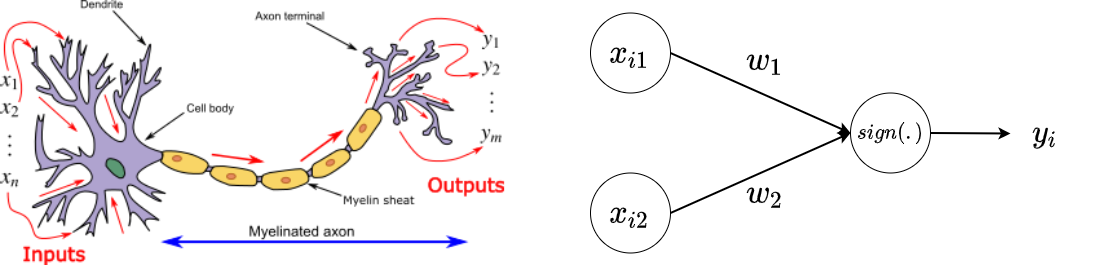
\includegraphics[width=\linewidth]{imgs_tomas/perceptron.png}
    \caption{Biological and Artificial neuron}
    \label{fig:neurons_comparison}
\end{figure}

To put the notation in context, let us present an example of the Perceptron architecture.
Imagine we have collected features $X \in R^{n \times d}$, where $n$ is the number of observations and $d$ is the number of predictors.
Based on these features, we would like to build a system capable of distinguishing if datapoint $x_i \in X$ comes from a dog ($y_i = 1$) or a cat ($y_i = -1$).
Our data point can, for example, consist of the weight of the animal and the length of the animal's nose.
Given this information, we can construct a Perceptron with 2 input neurons connected to 1 output neuron.
This architecture is depicted in Figure \ref{fig:neurons_comparison} on the right.

Formally, this architecture models the relation between $X$ and $Y$ according to the Equation \ref{eq:perceptron}. 

\begin{equation}
    y_i \sim h(x_{ij})= sign(\sum_{j=1}^{d} w_j \cdot x_{ij}) 
    \label{eq:perceptron}
\end{equation}

This modelling approach has 2 significant drawbacks.
First, it assumes the two classes are linearly separable by a hyperplane through the d-dimensional space induced by the predictors.
Second, it assumes the separation hyperplane goes through the centre of mass in the space.
To tackle the latter, we can introduce another parameter $b$, also called bias, to the equation.
The bias can be included as a weight of the edge from the bias neuron, which is a neuron always containing the value 1.
Therefore, we can treat this special case by using the general Equation \ref{eq:perceptron}.
Furthermore, the Equation \ref{eq:perceptron} can be simplified using the vector notation to Equation \ref{eq:perceptron2}.

\begin{equation}
    h(X) = sign(X \cdot W)
    \label{eq:perceptron2}
\end{equation}

To resolve the problem with linear separability, we can extend our model by using additional layers of neurons.
These additional layers are commonly called hidden layers of the neural network.
To be efficient, the hidden layers need to apply some non-linear function, also called the activation function.
The function modelled by this new network is of the form

\begin{equation}
    Y = sign(a_{k-1}(...a_2(a_1(X \cdot W_1) \cdot W_2)...\cdot W_{k-1}) \cdot W_{k}),
    \label{eq:perceptron3}
\end{equation}

where $a_l, l \in {1, ..., k}$ are the activation functions and $W_l, l \in {1, ..., k}$ are the weights of the connections corresponding to transition from layer $l-1$ to layer $l$.

There are many possibilities for the activation function and the choice of it usually depends on the particular goal in mind.
% from here it feels sloppy
Some of the most commonly used activation functions are listed in Figure \ref{list:activations} and visualized in the Figure \ref{fig:activation_functions}.

\begin{itemize}
    \item $\text{Identity}(x) = x$
    \item $\text{Tanh}(x) = \frac{\exp(x) - \exp(-x)}{\exp(x) + \exp(-x)}$
    \item $\text{Sigmoid}(x) = \frac{1}{1 + \exp(-x)}$
    \item $\text{HardTanh}(x) = \begin{cases}
             1 & \text{ if } x > 1 \\
             x & \text{ if } 1 \geq x \geq -1 \\
            -1 & \text{ if } x < -1 \\
          \end{cases}$
    \item $\text{ReLU}(x) = \max(0, x)$
    \item $\text{ELU}(x) = \max(0,x) + \min(0, \alpha * (\exp(x) - 1))$
    % \item $\text{Softmax}(x_{i}) = \frac{\exp(x_i)}{\sum_j \exp(x_j)}$
    \label{list:activations}
\end{itemize}

\begin{figure}
    \centering
    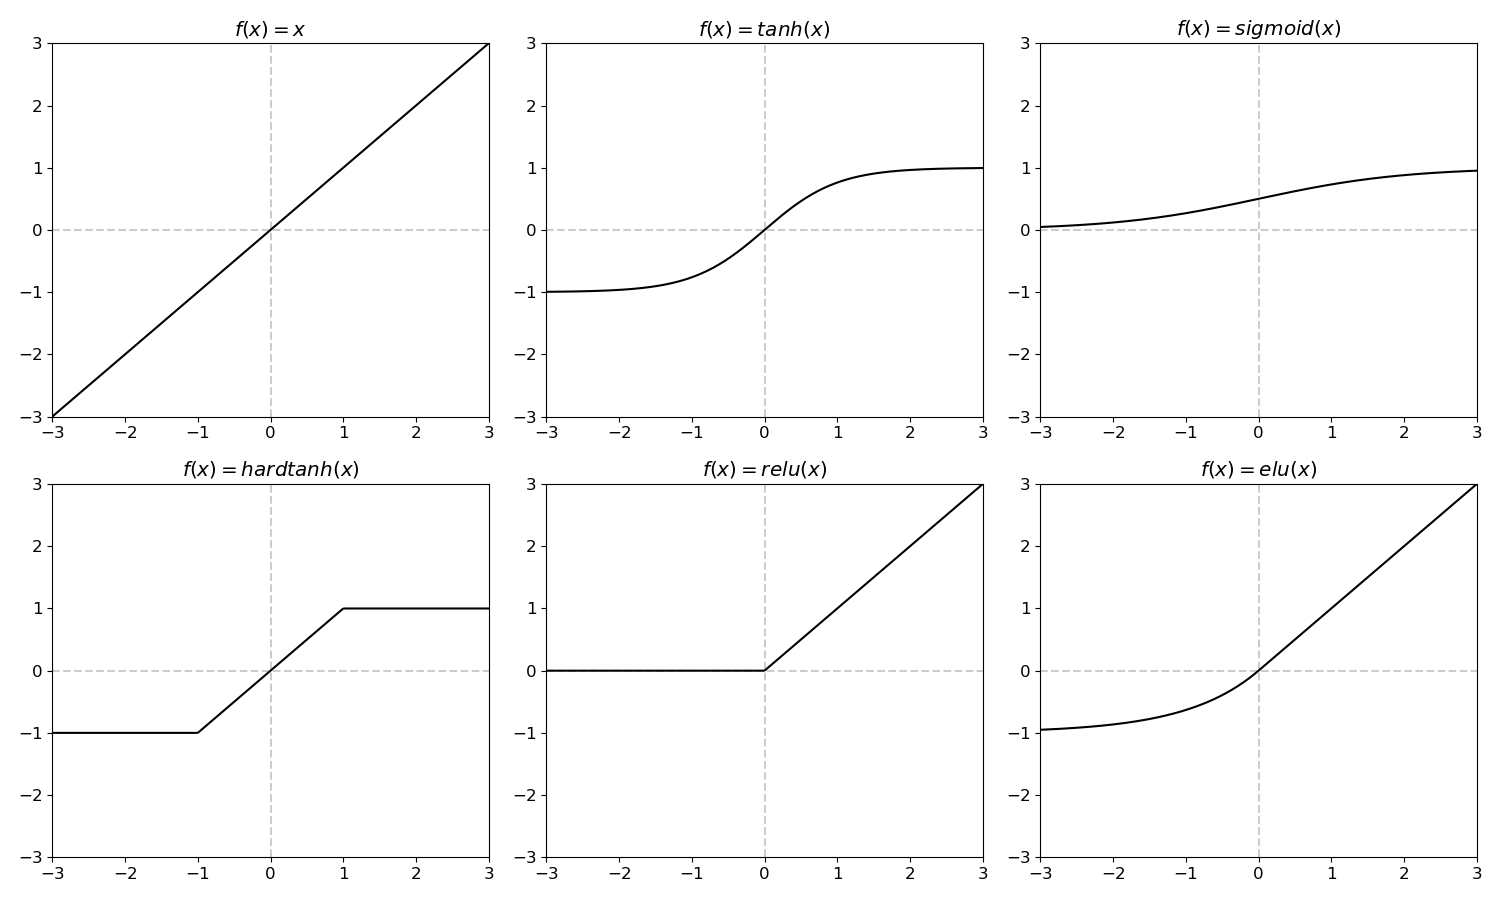
\includegraphics[width=\linewidth]{imgs_tomas/activation_functions.png}
    \caption{Activation Functions}
    \label{fig:activation_functions}
\end{figure}

% checkpoint
% softmax
% tanh(x) = 2*sigmoid(2x) -1

% https://ml-cheatsheet.readthedocs.io/en/latest/activation_functions.html
% In the single-layer Perceptron example, we already used a non-linear activation function on the output layer - the sign function.
Probably the first non-linear function to consider would be the sign function, since we already used this function in the output layer of the single-layer Perceptron.
Unfortunately, this function has a derivative 0 almost everywhere, with the exception of $x=0$ where it is non-differentiable and discontinuous.
These properties complicate the process of learning and therefore this function is rarely used during the training of the model.
To address these issues, researchers used hyperbolic tangents in the past as the smooth alternative to the sign function, sometimes scaling it to sigmoid function, which can be interpreted in probabilistic manner.
Unfortunately, these functions, although differentiable everywhere, often provide quite small gradients.
This creates a problem commonly called vanishing gradient.
% which we will discuss later in the section
Recently, a solution to this problem was proposed in the form of using Hard Hyperbolic Tangent (HardTanh) or the Rectified Linear Unit (ReLU).
These piecewise activation functions provide a gradients of 0 or 1, depending on the input values.
% dying ReLu problem
Finally, Exponential Linear Unit (ELU) is an improvement of the ReLU function which we use in this project. 
\subsubsection{Activation functions on output layer}
Until this point, we considered only the classification task with two classes.
However, it is possible to extend neural networks to much more different tasks at hand.
One of the possible extensions is the regression task, where our response is some numeric value $Y \in R^n$.
In these settings, we could use the Identity function on the output layer.
The error function, which we want to minimize would be an ordinary least squares. 

Another of the possible extensions is the multiclass classification task, where we want to learn to distinguish more classes.
In this case, we usually encode our output with one-hot-encoding.
For example, consider classification to 3 classes.
In this case, we can encode the labels as follows:
\begin{itemize}
    \item $1 \to (1, 0, 0)$ 
    \item $2 \to (0, 1, 0)$
    \item $3 \to (0, 0, 1)$
\end{itemize}
To enable our network to learn this relation, we use the output layer with 3 output neurons.
In theory, we could just use the Identity function and select the highest value as the predicted class, but in practice the Softmax function is often used.
The Softmax function is defined as:

\begin{equation}
    \text{Softmax}(x_{i}) = \frac{\exp(x_i)}{\sum_j \exp(x_j)}
\end{equation}

and it has some very nice properties.
Firstly, it maps the real-valued outcome to the interval $[0, 1]$.
Secondly, the sum of the outcome is always 1.
To be able to optimize a network with this output, we use the negative log likelihood loss.

\begin{equation}
    \ell(x, y) = \sum_{n=1}^N \frac{1}{\sum_{n=1}^N w_{y_n}} l_n 
\end{equation}

\subsubsection{Training of the neural networks}
The training of the neural networks refers to the learning process.
In neural networks, this is done by adjusting the weights $W$ in such a way that the relationship between input $X$ and output $Y$ is approximated as well as possible.
To be able to evaluate the performance of the current network, we need to define loss function.
This function gets the predicted output $\hat{Y}$ and the real output $Y$ and evaluates the error made during the prediction.
Some commonly used loss functions are, for example, Mean Squared Error (MSE) and the Negative Log-Likelihood.
The Mean Squared Error is mainly used in regression setting, when we want to predict a continuous value.
It is defined by equation \ref{eq:MSE}.

\begin{equation}
    \ell(\hat{Y}, Y) = \text{mean}(L) = \text{mean}(l_1,\dots,l_N), 
    \text{where} l_n = (\hat{Y}_n - Y_n)^2
    \label{eq:MSE}
\end{equation}

The Negative Log-Likelihood is used for classification purposes with C classes.
It is defined by equation\ref{eq:NLL}.
% NLL = -log(p), nie? toto je trochu matuce, aj s tym MSE hore
\begin{equation}
    \ell(\hat{Y}, Y) = \sum_{n=1}^N \frac{1}{\sum_{n=1}^N w_{Y_n}} l_n,
    l_n = - w_{y_n} x_{n,y_n},
    \label{eq:NLL}
\end{equation}

The input to this loss function has to contain log-probabilities of each considered class.
Obtaining log-probabilities from the neural network can be achieved by adding Softmax activation function to the output layer and taking logarithm of the resulting values.

Now, with all parts in place, we can illustrate the training process.
The training of the neural networks is done iteratively.
First, we predict the output values $\hat{Y}$ for our input $X$.
This is done in the forward pass through our neural network.
Afterwards, we calculate the error using the loss function.
Then, we use this error to calculate the gradient with respect to weights.
This is done in the backward pass through our neural network.
The weights are then updated in the direction of negative gradient.
The process is then repeated, until convergence is achieved.

This training process is also referred as Gradient Descent and we provide the algorithm in the Box \ref{alg:gd}.

\begin{algorithm}
\caption{Gradient Descent}
\label{alg:gd}
\begin{algorithmic}[1]
\State $w \gets \textit{initialize}$
\Repeat
\State $\hat{Y} = \textit{predict(X, w)}$
\State $w = w - \alpha * \nabla_w E_{in}(\hat{Y}, Y)$
\Until{convergence}
\end{algorithmic}
\end{algorithm}

Although this algorithm provides a solid basis to analyze the learning process, it is usually too slow to be used in practice.
This is mainly caused by the need to calculate the predictions across all the datapoints in the training dataset.
Since nowadays the training datasets tend to be very big, a modification to this algorithm was proposed.
Instead of using all the datapoints from training dataset, the error is just estimated with one point.
This is what is called the Stochastic Gradient Descent and it was one of the most significant steps in adopting the neural networks in a broad range of tasks.

The time complexity of the Gradient Descent is $\mathcal{O}(n\log{\frac{1}{\epsilon}})$, where $n$ is the number of datapoints in the training dataset and $\epsilon$ is how far away from the minimum we want to end up.
As we can see, the $n$ factor in this time complexity is very significant when the dataset is huge.
Because the Stochastic Gradient Descent uses just one datapoint to estimate the gradient, it makes noisy estimates, which might not be in the optimal direction, but it is able to make those estimates much more quickly.
The time complexity of this method is $\mathcal{O}(1\cdot\frac{1}{\epsilon})$.

In practice, we prefer to use more datapoints than one during the training to estimate the gradient.
This is called the Mini-Batch Stochastic Gradient Descent and it presents a middle-ground option between the two extremes.
The estimates of the gradient are not as noisy as during the SGD and the time to compute the gradient is also significantly reduced. 

\subsubsection{Parameter initialization}
Another important aspect of the neural networks is their parameter initialization.
A naive solution would be to initialize them to 0 and let the network learn the true weights.
Unfortunately, this naive solution would be a terrible one, because it would cause the neural network to update all the weights the same way.
Therefore, we usually initialize the weights to some random weights.
This ensures to break the symmetry during the learning and allows to update the weights efficiently.

Another thing to consider is the magnitude of these newly initialized weights.
Too big or too small values can cause numerical issues during the training due to limitations of float number representation in computers, which are inherently discreet systems.
Initializing the weights to sample from Uniformly distributed values from interval [0, 1] or from Normal distributed values with mean 0 and standard deviation 1 usually works fine for smaller neural networks, but might cause numerical problems when the number of input connections and the number of output connections is big.
Therefore, an improved aproaches, which take number of incomming and outgoing connections, were proposed.
First approach is the Glorot initialization \cite{glorot2010understanding}.
In this initialization, the weights are sampled either from an Uniform distribution from interval [$-a, a$] or from Normal distribution with mean 0 and standard deviation $a$, where parameter $a$ is defined as:

\begin{equation}
    a = \text{gain} \times \sqrt{\frac{6}{\text{fan\_in} + \text{fan\_out}}}
\end{equation}

Another approach is the He initialization \cite{he2015delving}.
This initialization is very similar to Glorot initialization and the only difference is in the calculated value of the parameter.
In the case of Uniform distribution, the boundary parameter is calculated by

\begin{equation}
    \text{bound} = \text{gain} \times \sqrt{\frac{3}{\text{fan\_mode}}},
\end{equation}

and in the case of Normal distribution, the standard deviation parameter is calculated by

\begin{equation}
    \text{std} = \frac{\text{gain}}{\sqrt{\text{fan\_mode}}}.
\end{equation}
% this needs more explanation

\subsection{Convolutional Neural Networks}
Convolutional neural network (CNN) is a special type of neural network designed to work with data with a strong spatial dependence.
One canonical example of such data are images.
The strong spatial dependence in the image data is demonstrated by the fact that often the regions close to each another exhibit the same values of the pixel colors.
Another important feature of the image data is the translational invariance, meaning that an object moved from one position in the picture to another position is still identifiable.

A basic operation in the convolutional neural networks is the convolution.
The convolution operation is inspired by the experiments on cat's visual cortex performed by Hubel and Wiesel \cite{hubel1959receptive}.
Here, the biological neurons are divided into small regions which differ in sensitivity towards the stimuli from different regions of visual field.
Furthermore, the sensitivity of different regions varies with the different shape and orientation of the observed objects.
For example, a vertical lines in the visual field can activate some regions of the biological neurons and horizontal lines can activate different regions of the biological neurons.
The regions are then connected in hierarchical fashion, which allows the deeper regions to recognize for example squares.

% add: locality 
Convolutional neural networks are using similar principles to extract and encode an important features of presented image.
From the computational point of view, CNNs are neural networks heavily regularized by the number and location of connections.
They perform exceptionally well on image classification tasks, recently achieved human-level performance on ImageNet dataset.
The ImageNet dataset is the benchmark dataset used in ImageNet Large Scale Visual Recognition Competition (ILSVRC), which is annual competition hugely contributing to the development and application of neural networks.
% imagenet uz nebezi. Zacne sa prechadzat z 2d na 3d - kukni objectnet
% add:
% different architectures, with just minor changes
% some notable winners - LeNet, AlexNet, 

\subsubsection{Convolution layer}
% add: CNN defined as neural netowkrs with at least one convolutional layer 
Convolution layer is the characteristic unit of the Convolutional Neural Network.
It applies the Kernel to the data to transform the input to the output.
The Kernel is a small grid with trainable parameters.
To illustrate how to apply such a Kernel to the data let us imagine a Kernel $K$ with the size $3 \times 3$.
In this example, we will apply this to an image $I$ of size $5 \times 5$ pixels, where each pixel contains one numerical value, representing the brightness of the pixel.
First we will apply the Kernel to the image at position $(0, 0)$.
This means, we will do element-wise multiplication between the Kernel and the part of the Image from position 0 to position 3 on x-axis and from position 0 to position 3 on y-axis.
Afterwards, we will sum all the products of the multiplication to get a first result of the convolution process with position (0, 0).
Then, we will move the Kernel by one pixel to the right.
Here, we will perform the same operation, with the only difference that the part of the Image used in this convolution will start at position 1 on the x-axis and 0 on the y-axis.
The result of this convolution will be assigned to the position (1, 0) as well.
We continue the operation by shifting the Kernel to the right until we reach the end if the Image.
Afterwards, we will shift the Kernel by one pixel down and start the same process of convolution on this row.
This is repeated until we slide through all possible rows and columns of the Image grid.
The convolution operation is visualized in Figure \ref{fig:convolution}.

% tento obrazok je zbytocny podla mna. nedodava viac informacie ako ten pod nim, ktory este zahrnuje aj padding a stride. a zabera vela miesta
\begin{figure}
    \centering
    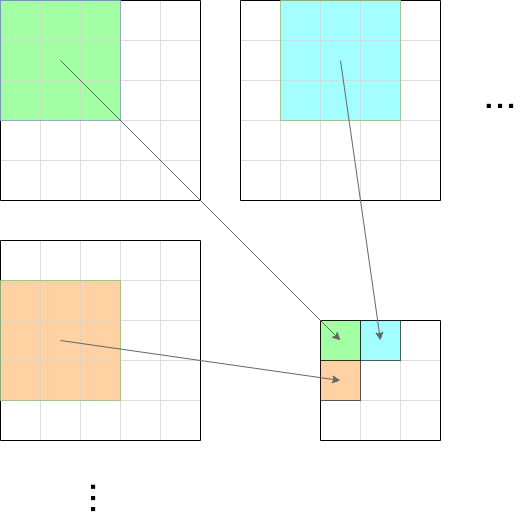
\includegraphics[width=\linewidth]{imgs_andy/convolution.png}
    \caption{Convolution operation}
    \label{fig:convolution}
\end{figure}

% padding
An important observation in this case is that the convolution operation reduces the size of the image by default.
This behaviour is usually not desirable, because it might lead to loss of information at the edge of the image.
Fortunately, it can be easily corrected by using a padding.
Using the padding results in adding some number of pixels, usually containing zeros, to the edge of the image.
In our example, we could extend the Image from $5 \times 5$ to $7 \times 7$ by adding zeros around it.
This would ensure, that the dimensionality of the picture stays the same after convolution.

% half-padding
The size of the padding mainly depends of the size of the selected kernel.
Some of the most used kernel sizes are $3 \times 3$, $5 \times 5$ and $7 \times 7$, with their corresponding paddings $1$, $2$ and $3$.
In general, the padding preserving the size of the image is of size $(F_q - 1)/2$ pixels wide.
This type of padding is also called half-padding, because almost half of the kernel is sticking out of the original image at the edges.

% valid padding
Using the half-padding usually works better in experiments than using no padding, which is sometimes also referred as valid padding.
The intuition behind this remark is that valid padding tends to under-represent the information at the borders in comparison with the central pixels of the image.
Due to these disadvantages of the valid padding, it is rarely used in practice and most of the architectures tend to use the half-padding.

% full padding
Another type of padding is the full-padding.
In this case, we will pad the image with border of $F_q - 1$ zeros wide.
This padding allows almost the full kernel to stick out of the image.
One interesting remark about this type of padding is that every pixel of the original image is covered same number of times.
Furthermore, this padding increases the dimensions of the image by $F_q - 1$.
To illustrate the reason why, let us consider the image of size $(W, H)$.
This image will be padded by $F_q - 1$ from all sides, therefore the size of the padded image will be $(W + 2\cdot(F_q - 1), H + 2\cdot(F_q - 1))$.
After convolution, this padded image will be reduced to $(W + F_q - 1, H + F_q - 1)$, therefore it is bigger by $F_q - 1$ in every dimension in comparison to the original image.
This fact is sometimes used in "reverse" convolution layers, which are mainly used in different autoencoder architectures.

\subsubsection{Strides}
Until now, we considered two parameters of a convolution layer - kernel size and padding.
Another parameter sometimes used in convolution layers is stride.
The stride correspond to the shift by which we move the kernel along the axis.
In the previous example, we used the stride of $1$.
Using the bigger values for stride $S$ has an effect of reduction of the dimension of the image by a factor of approximately $S$. 
To clarify how this is done, let us consider the movement on the x-axis in the previous example.
There, we started at the position 0, then continued with position 1, followed by position 2 and so on.
This can also be written as a sequence $0\cdot S, 1\cdot S, 2\cdot S\dots$ with the stride parameter $S = 1$.
By increasing the stride parameter to 2, we would get a sequence $0\cdot2, 1\cdot2, 2\cdot2\dots = 0, 2, 4\dots$.
This is also shown in Figure \ref{fig:stride}

\begin{figure}
    \centering
    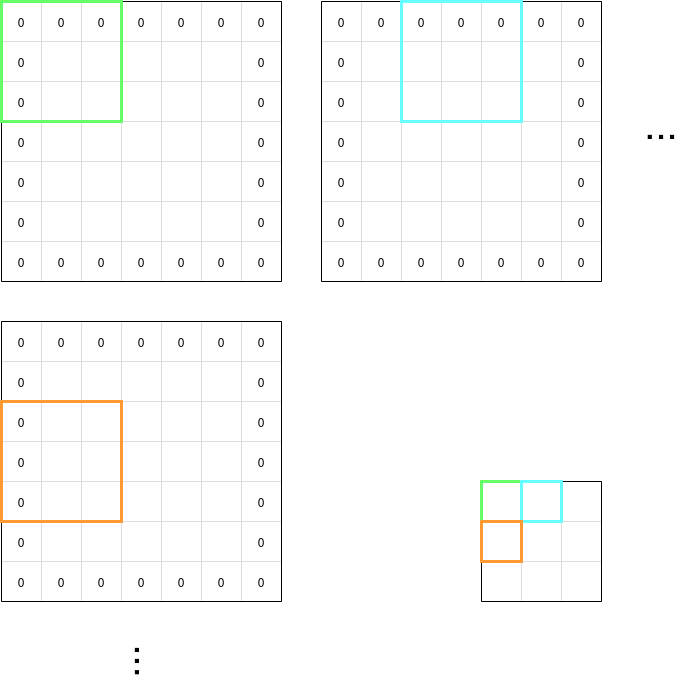
\includegraphics[width=0.6\linewidth]{imgs_andy/stride.png}
    \caption{Convolution with half-padding and stride 2}
    \label{fig:stride}
\end{figure}

It is noteworthy, that increased stride reduces the dimensions of the image.
This effect is even stronger than reduction of the dimensions by valid padding, but it does not suffer by under-representing data closer to the border.
In general, it reduces the size of the image according to the Equation \ref{eq:stride}, where $L_1$ is the length of the dimension when using the stride $S=1$ and $S$ is the used stride.

\begin{equation}
    L_S = \floor*{L_1 / S}
    \label{eq:stride}
\end{equation}

Sometimes, this reduction is even used as an advantage, especially, when the resolution of the image is too high.
It can also help to reduce over-fitting or in cases, when the memory is constrained.
Another remark is that the stride increases the receptive field of the consequent convolutions.
This allows the consequent convolutions to capture more complex features in the deeper layers.
A similar function is performed by another characteristic layer of Convolutional Neural Networks presented in the following part.

\subsubsection{Pooling layer}
Similarly to the Convolution layers, Pooling layers operate on small regions of the Image.
There are two main difference between these two types of layers.
First difference is that the pooling layer usually uses the stride parameter $S$ of the same value than the size of the kernel in that particular direction.
The second difference is that the pooling layer does not use the dot product.
The most common practice is to take the maximum of the entry-wise product.
This is referred as max-pooling.
Additionally, pooling can use any other function, which takes the matrix of entry-wise products and returns a single number, like for example average.
These other functions are rarely used, mainly due to their worse performance in practice. 

The main purpose of the pooling layers in Convolutional Neural Networks is to increase the receptive field in the consecutive layers, while decreasing the spatial size.
A similar effect can be accomplished with strided convolutions, which sometimes makes pooling layers unnecessary.
Nevertheless, the effect of max pooling can not be exactly replicated due to the max operation.

\subsubsection{Dilated convolutions\cite{yu2015multi}}
% https://towardsdatascience.com/review-dilated-convolution-semantic-segmentation-9d5a5bd768f5
As we saw in previous examples, the standard convolutions take into account a region of the input image and perform the convolution operation with the kernel.
This region usually consists of a few consecutive pixels in the x-axis and y-axis.
A relatively recent innovation is to consider as a region pixels separated by a few skipped pixels.
This is shown in the Figure \ref{fig:dilated_conv}.

\begin{figure}
    \centering
    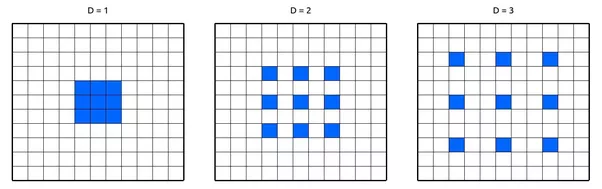
\includegraphics[width=\linewidth]{imgs_andy/dilated_conv.png}
    \caption{Dilated convolutions}
    \label{fig:dilated_conv}
\end{figure}

This is called dilated convolutions and effectively it increases receptive field of the convolution operation.
Formally, the output of convolution at position $i, j$ of input map can be calculated as:

\begin{equation}
    \text{OUT}_{i,j} = \sum_{k=0}^{K-1} \sum_{l=0}^{K-1} \text{IN}_{i+(k \cdot D),j+(l \cdot D)} \cdot \text{KERNEL}_{k, l},
\end{equation}

where $K$ is the kernel size and D is the dilation.

% local connectivity - the neuron will be connected only to small number of neurons in the previous layer, which are close together
% part of the image that the neuron is connected to is called receptive field
% The receptive field is defined as the region in the input space that a particular CNN’s feature is looking at (i.e. be affected by)
% https://medium.com/mlreview/a-guide-to-receptive-field-arithmetic-for-convolutional-neural-networks-e0f514068807

\subsubsection{Convolutions through multiple channels}
% basic principle
Up to this point, we have considered only convolutions on maps with only one channel.
Examples of such maps are for instance gray scale images, where each grid entry contains one number representing the intensity of light in that particular pixel.
However, commonly the images we want to process consist of pixels with 3 different channels.
Such images can then be represented in a 3-dimensional tensor of $W \times H \times C$, where $W$ is the width of the picture in pixels, $H$ is the height of the picture and $C=3$ is the depth used to store intensities of 3 basic colors - red, green and blue. 

In this case, the convolution is performed similarly to the convolution in the simple case, only now our kernel is of size $K \times K \times 3$.
The computation of the output value is shown in the Equation \ref{eq:conv_channels}.

\begin{equation}
    \text{OUT}_{i,j} = \sum_{k=0}^{K-1} \sum_{l=0}^{K-1} \sum_{m=0}^{C-1} 
        \text{IN}_{i+k,j+l, m} \cdot \text{KERNEL}_{k, l, m}.
    \label{eq:conv_channels}
\end{equation}

Often, it is desired to transform the input with multiple channels to output with multiple channels, where the output channels capture different features of the Image.
This is done using multiple kernels where each kernel produces a single map of some specific features.
For example, we can have one kernel which is able to detect edges of the objects in the image and another kernel which is able to detect texture of the objects.
To incorporate these options, PyTorch framework allows to initialize the convolution layers with parameters $\text{in\_channels}$, $\text{out\_channels}$, $\text{kernel\_size}$, $\text{padding}$, $\text{stride}$, $\text{dilation}$.

% 1X1 convolution
One special convolution operation is noteworthy at this point, commonly referred to as $1 \times 1$ convolution.
This convolution uses kernel of size $1 \times 1$ and therefore would not do anything significant in the settings with one input map and one output map.
However, in the settings with multiple input and output channels, this operation can be used to change the number of maps representing our data.

% groups
Another useful modification to the convolution operation is using $\text{groups}$.
By default, this parameter is usually set to $1$, which means that only one group is created from all input channels, to create an output map.
By, for example, setting this parameter to $2$, $2$ groups would be created from input channels.
First half of the input channels would create one map and the second half of the input channels would create the second one.
If the groups parameter is set to the number of input layers, each input layer is used separately to create one output layer.
This setting is mainly useful in combination with $1 \times 1$ convolutions, where it can reduce the number of parameters significantly. 

% reduction of the parameters using the 1X1 convolution
To illustrate the reduction of parameters, let us imagine that the input has $N$ channels and the output has $M$ channels.
To perform a classical convolution with kernel size $K \times K$ we would need $K \cdot K \cdot N \cdot M$ parameters.
We can reduce this number, by first applying $1 \times 1$ convolution, followed by convolution with $\text{groups} = M$.
This way, the number of needed parameters is $1 \cdot 1 \cdot N \cdot M + K \cdot K \cdot M$.

For example, performing $3 \times 3$ convolution with $3$ input channels and $2$ output channels would require 54 parameters with classical convolution and only 24 parameters using the $1 \times 1$ followed by grouped convolution.

Of course, these two operations are not identical, but it can be argued they serve the same intended purpose.
The intended purpose of the depth in basic convolution is to use the information from multiple channels.
In the reduced approach, this is delegated to the $1 \times 1$ convolution.
The kernel size greater than one in basic approach is used to capture the locality of the features.
In the reduced approach, this responsibility is passed on the grouped convolution. 

\subsection{Residual Neural Networks}
A great portion of improvement of accuracy of the recent neural network models is based on the increased computational power, availability of huge data sets and changes in the architecture of the models.
The prevalent trend is to use deeper neural networks, because they tend to perform better in practice.
This can be intuitively explained by the hierarchical nature of the features extracted.

Unfortunately, the increased depth of the model is also usually linked with the problems of vanishing and exploding gradients.
To overcome this issues a new architecture was proposed - residual neural network.
This architecture introduces skip connections between the layers. 
The main idea of these skip connections is to let the network decide of the depth that is needed to model a specific feature.
To show why this is needed let us consider an image containing two object with very different complexity - for instance a human face as an object of relatively high complexity and a simple geometrical shape such as triangle as an object of relatively low complexity.
To model the human face well, it is likely that a deeper neural network would be needed due to the number of small details which we need to capture.
On the contrary, to model a simple triangular shape a shallow network is likely to be sufficient.
In residual networks the skip connections allow to model both regions of the image using the same network.
In the case of face modelling the network will use the deep layers to capture the details and in the case of the triangle only a first few layers will be used and most other layers will be skipped using the skip connections.

The skip connections are realized through addition of the identity to the output of a particular layer.
This is visualized in the Figure \ref{fig:skip_connection}.
\begin{figure}
    \centering
    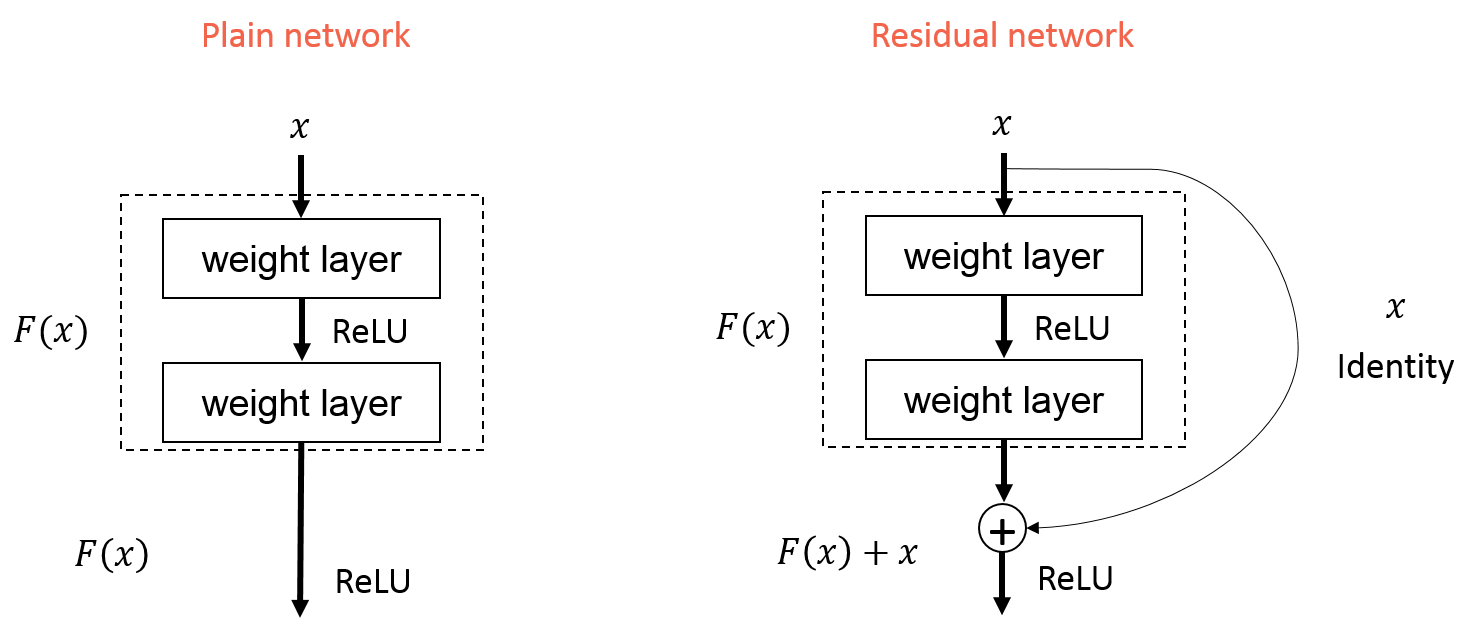
\includegraphics[width=\linewidth]{imgs_andy/skip_connection.png}
    \caption{Skip connection}
    \label{fig:skip_connection}
\end{figure}
These skip connections provide an alternative way for the flow of gradient.
The shortest path, the path using most skips, is learning the most important features of the input.
The longer paths can then be intuitively viewed as a residual contributions \cite{he2016deep}.
For this reason, residual networks tend to be more robust to the choice of depth of the model.
    
% \subsection{AlphaFold}

\newpage

\section{Structure Realization}

\begin{figure}[b]
    \centering
    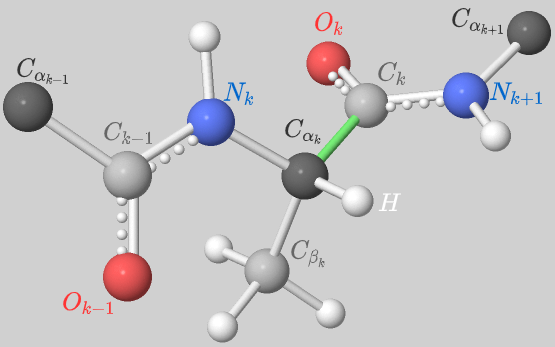
\includegraphics[scale=0.5]{imgs_tomas/backbone.png}
    \caption{Protein backbone with atom names. Modified picture from \cite{ramachandran}}
    \label{fig:backbone}
\end{figure}

The structure realization step refers to a process of optimizing three-dimensional conformation of protein according to some constraints or energy/potential function. 
If we assume that the bond length between neighbouring atoms in the backbone (atoms N, C$_\alpha$ and C) + C$_\beta$ atom is constant as well as the angle between atoms in the same plane (angles N-C$_{\alpha}$-C, C$_{\alpha}$-C-N, C-N-C$_{\alpha}$) then the entire structure can be fully described by a set of three torsion angles $\phi$, $\psi$ and $\omega$.

This assumption allows us to create a model of protein geometry $\mathcal{G}(\phi, \psi)$ that can be optimized ($\omega$ is almost always 180\degree, and so was treated as a constant). 

In the following sections, we will describe how we tackled the protein geometry problem, together with the explanation of torsion angles and how to calculate atom coordinates from them and a short recap of basic linear algebra operations that were used.

\subsection{Torsion Angles to Coordinates}

% \begin{figure}
%     \centering
%     % 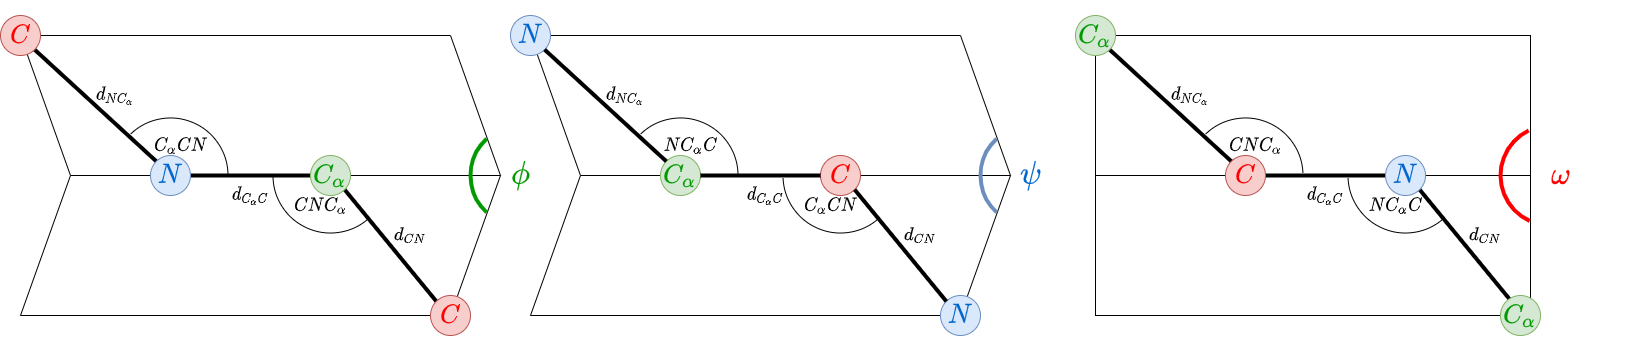
\includegraphics[scale=0.27]{imgs_tomas/torsion.png}
%     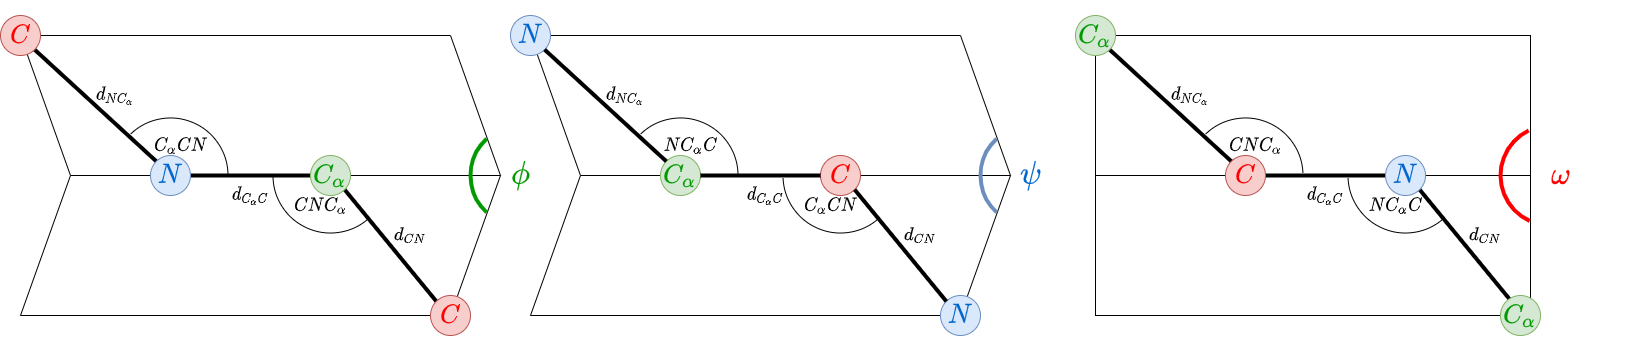
\includegraphics[width=\linewidth]{imgs_tomas/torsion.png}
%     \caption{Torsion Angles - planes and inter-atom distance and angles notation}
%     \label{fig:torsion}
% \end{figure}

% Torsion angle, or a dihedral angle, is an angle defined by two intersecting planes. A protein is essentially composed of a sequence of aminoacids, where every aminoacid contains atoms N, C$_\alpha$ and C and almost all (except of glycine) contain a C$_\beta$ atom with a residue.
% The C$_\beta$ has a bond with the C$_\alpha$ atom - Figure \ref{fig:backbone} depicts the individual atoms of the backbone together with C$_\beta$ atom.

% Since there are three atoms in the backbone, we can define three pairs of intersecting planes and thus define the three torsion angles (Figure \ref{fig:torsion}). Knowing the position of three preceding atoms, the torsion angle $\phi$ defines the position of the next C atom, the torsion angle $\psi$ defines the position of the next N atom and finally $\omega$ defines the position of the next C$_\alpha$ atom. The bond between atom C and N in the protein backbone is a peptide bond that behaves similarly to a double bond and is almost always equal to 180\degree~(trans isomerism; 0\degree~for cis configuration).

Seeing that essentialy each torsion angle defines a position of an atom in relation to the previous three atoms in the structure, which are placed in a single plane, we can simplify the problem to follwing steps:

\begin{enumerate}
    \item Place the atom in the same plane as the previous three atoms, satisfying the inter-atom angles and distances (eg. for placing atom N$_1$, we need to know position of N$_0$, C$_{\alpha 0}$ and C$_0$ and angles NC$_\alpha$C and C$_\alpha$CN).
    
    \item Define a vector $\bm{v}$ as the difference between the coordinates of the new atom and the last atom in the structure (eg. $\bm{v} = $N$_1$ - C$_0$).
    
    \item Define a unit vector $\bm{k}$ around which the vector $\bm{v}$ will be rotated. This vector lies at the intersection of the two planes (eg. $\bm{k} = \frac{\textrm{C}_0 - \textrm{C}_{\alpha 0}}{d_{\textrm{C}_{\alpha} \textrm{C}}}$)
    
    \item Rotate the vector $\bm{v}$ around an axis with unit vector $\bm{k}$ and move it by adding the coordinates of the last atom in the structure
\end{enumerate}

These steps will be described in further detail in following section. Figure \ref{fig:bond_rotation} visualizes the steps except of the vector translocation.

% !!! REDO !!!
\begin{figure}
    \centering
    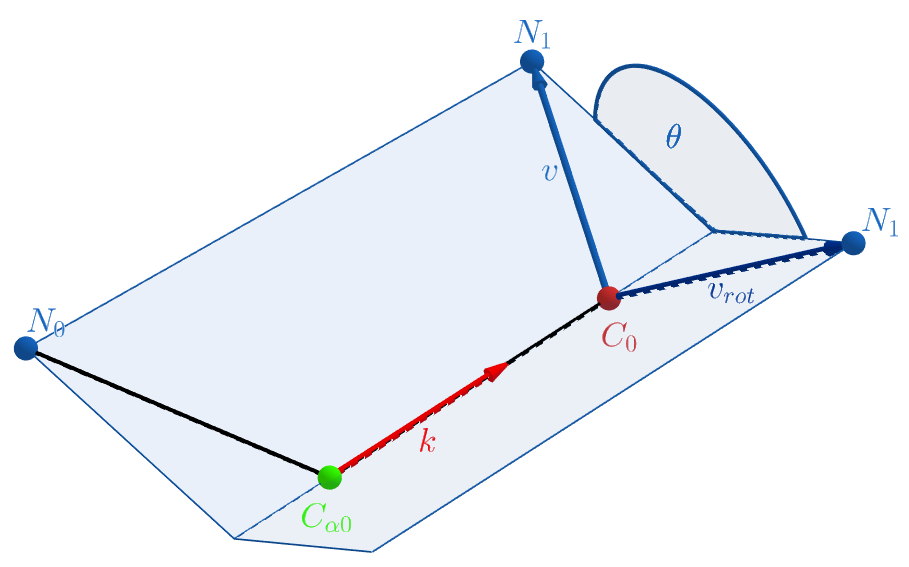
\includegraphics[scale=0.28]{imgs_tomas/rodrigues_backbone.png}
    \caption{Torsion angle rotation as vector rotation}
    \label{fig:bond_rotation}
\end{figure}

\subsection{Background - Vector Cross-product}

The cross product $\bm{v} \times \bm{w}$ of two 3D vectors is a vector pointing to a direction perpendicular to both vectors (decided by the right hand rule, where if $\bm{v}$  is represented by a thumb and $\bm{w}$ as index finger, than the direction is given by the middle finger). The size of this vector is equivalent to the area of the parallelogram with sites of sizes $||\bm{v}||$ and $||\bm{w}||$.

Formally the cross-product is a determinant of a special matrix with first column being the unit vectors $u_x$, $u_y$ and $u_z$ of the cartesian coordinate system and the rest are vectors $\bm{v}$ and $\bm{w}$:

$$\bm{v} \times \bm{w} = det
\left(
\begin{array}{ccc}
    u_x & v_{x} & w_{x}\\
    u_y & v_{y} & w_{y}\\
    u_z & v_{z} & w_{z}\\
\end{array}
\right) = ||\bm{v}||~||\bm{w}||~sin(\alpha)~\bm{n}
$$

where $\alpha$ is the angle between the two vectors and $\bm{n}$ is the unit normal vector perpendicular to both vectors.

\subsection{Background - Vector Dot-product}
% \begin{figure}
%     \centering
%     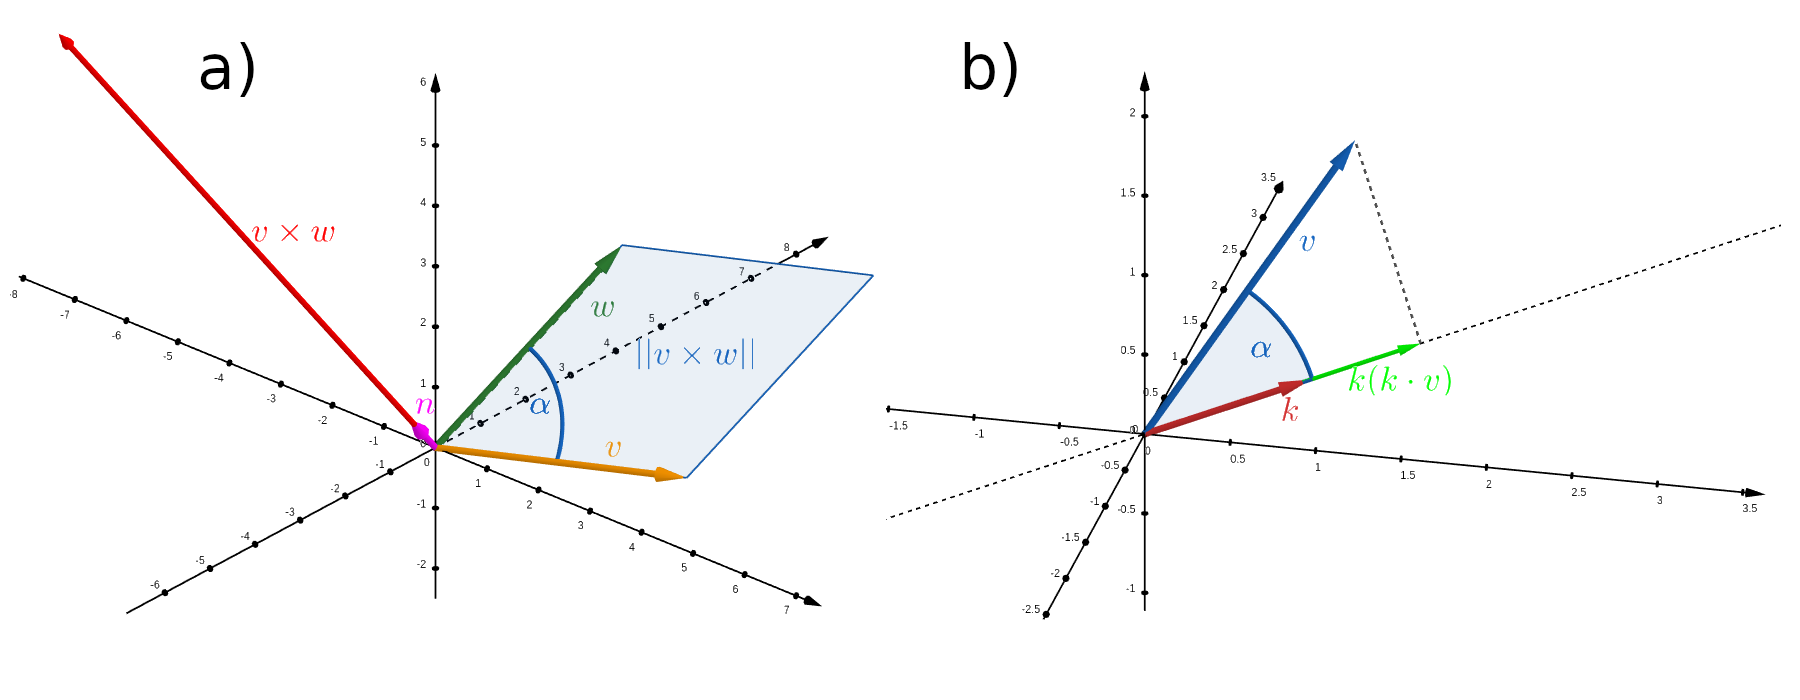
\includegraphics[scale=0.23]{imgs_tomas/vector_ops.png}
%     \caption{Visual demonstration of vector cross-product - a) and scalar/dot product - b)}
%     \label{fig:vector ops}
% \end{figure}

The dot product $\bm{k} \cdot \bm{v}$ is an operation that projects vector $\bm{v}$ onto a line defined by vector $\bm{k}$ and then scales the projection by the size of vector $\bm{k}$. In the special case when $\bm{k}$ is a unit vector, the result is a simple projection. Formally:

$$\bm{k} \cdot \bm{v} = ||\bm{k}||~||\bm{v}||~cos(\alpha) = k_x v_x + k_y v_y + k_z v_z$$

where $\alpha$ is the angle between the two vectors.

\subsection{Vector Rotation}

\begin{figure}
    \centering
    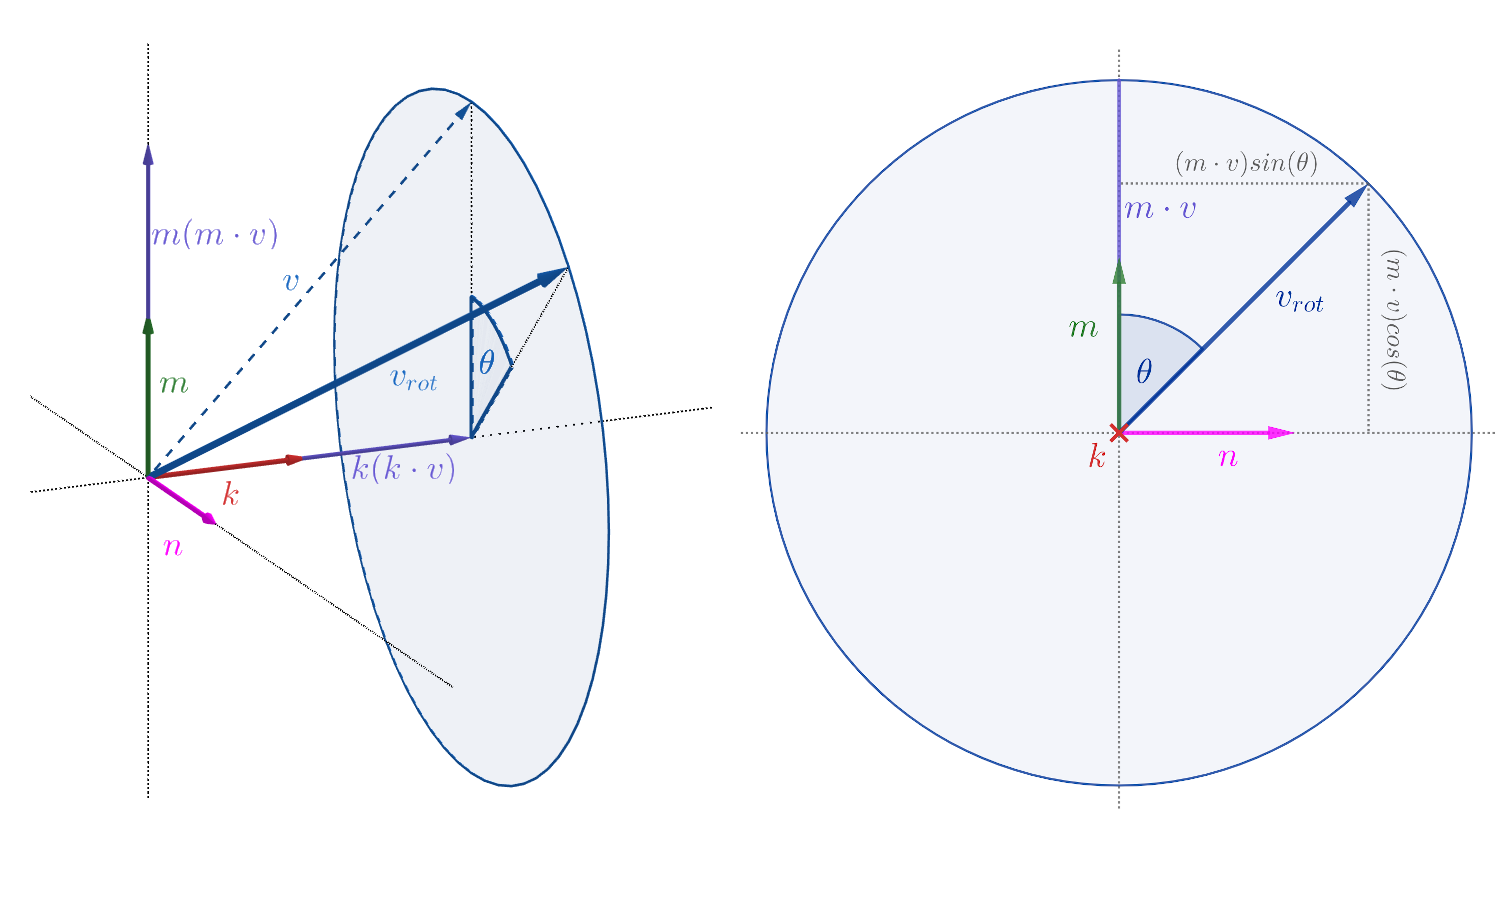
\includegraphics[scale=3]{imgs_tomas/rodrigues_3d2d.png}
    \caption{Caption}
    \label{fig:rodrigues3d2d}
\end{figure}

Lets assume that there is a vector $\bm{v}$ and a vector $\bm{k}$. Our task is to find vector $\bm{v_{rot}}$ which is a rotated version of vector $\bm{v}$ around a line defined by vector $\bm{k}$. Figure \ref{fig:rodrigues3d2d} depicts all the vectors and operations used in the following paragraphs.

The first step is to redefine the coordinate system in terms of 3 unit vectors: one is vector $\bm{k}$, second is a vector perpendicular to both $\bm{k}$ and $\bm{v}$: $\bm{n} = \frac{\bm{k} \times \bm{v}}{||\bm{k} \times \bm{v}||}$ and third a vector perpendicular to both $\bm{n}$ and $\bm{k}$: $\bm{m} = \bm{n} \times \bm{k}$.

\begin{enumerate}
    \item "$\bm{k}$ axis"
    
    The new rotated vector will always be the same distance away in the $\bm{k}$ vector direction. The amount is the projection of $\bm{v}$ onto $\bm{k}$, which is $\bm{k} \cdot \bm{v}$.
    
    \item "$\bm{n}$ axis"
    
    The amount by which we need to scale the unit vector $\bm{n}$ is the $sin(\theta)$ multiplied by the radius of the circle in the Figure \ref{fig:rodrigues3d2d}. The radius of the circle is a dot product of vector $\bm{m}$ and the initial vector $\bm{v}$.
    \item "$\bm{m}$ axis"
    
    The same reasoning as above, but this time the radius has to be multiplied by the cosine of $\theta$.
\end{enumerate}

All together, the rotational formula is:

\begin{equation}
    v_{rot} = \bm{k}(\bm{k} \cdot \bm{v}) + \bm{n} (\bm{m} \cdot \bm{v}) sin(\theta) + \bm{m} (\bm{m} \cdot \bm{v}) cos(\theta)
    \label{eq:rotformula}
\end{equation}

\subsection{Beta carbon atom placement}
% $C_{\beta}$

\begin{figure}
    \centering
    % 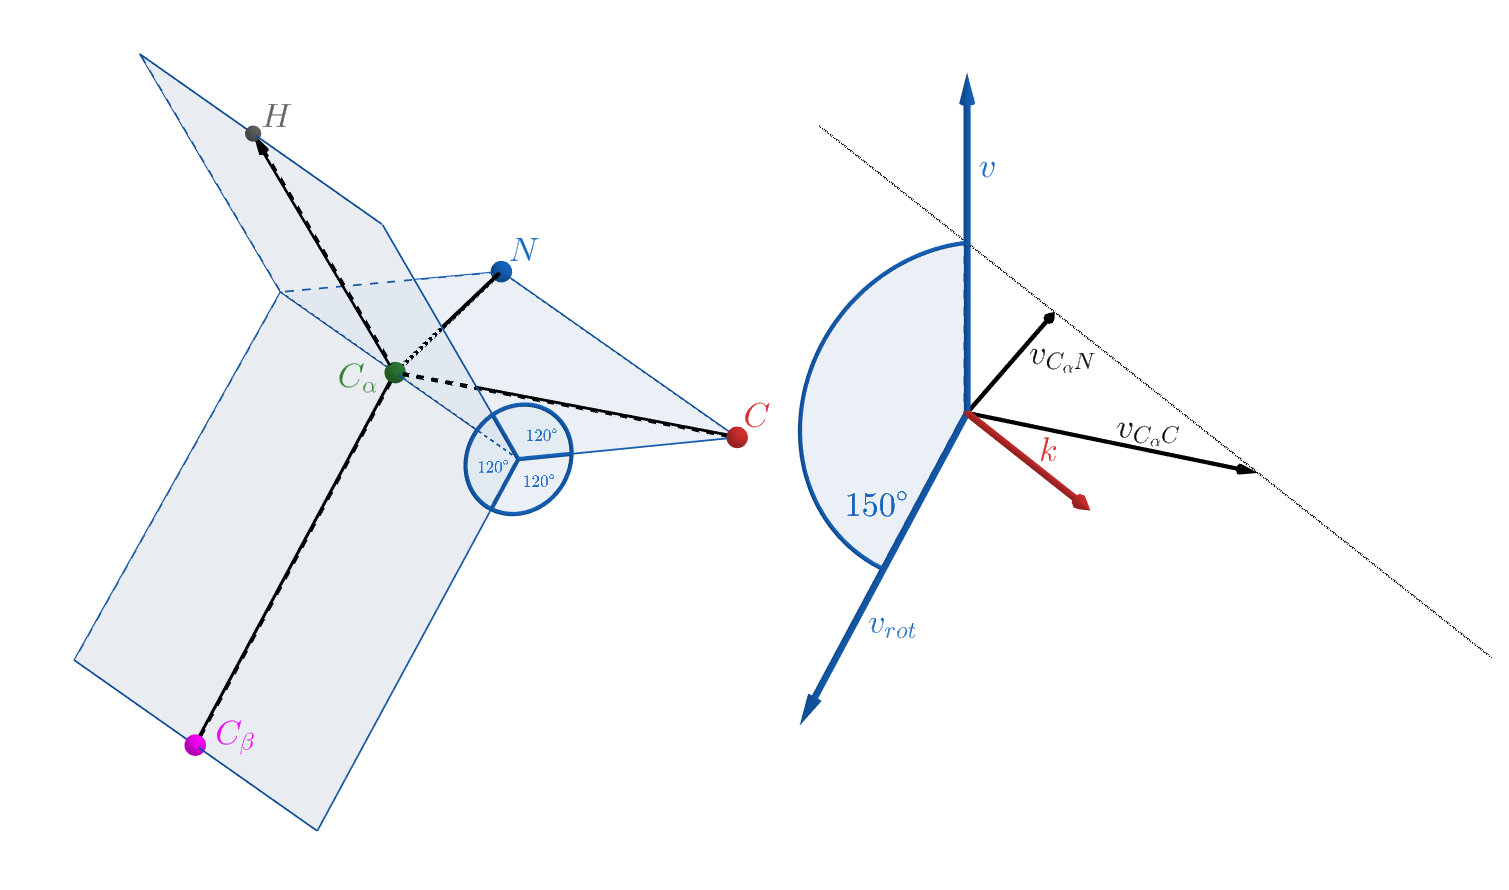
\includegraphics[scale=0.25]{imgs_tomas/cbeta.png}
    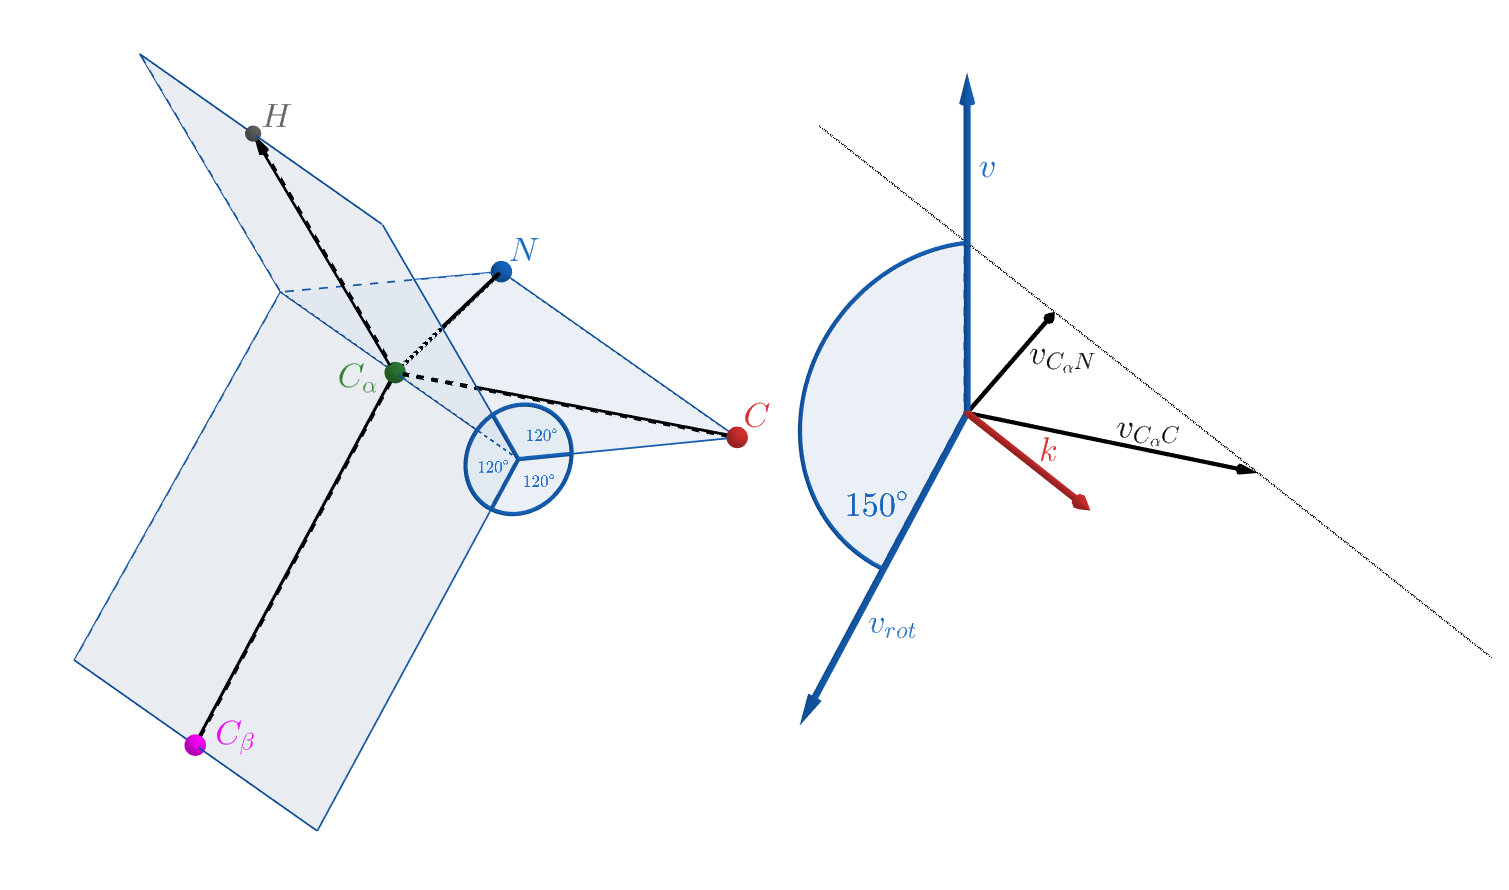
\includegraphics[width=\linewidth]{imgs_tomas/cbeta.png}
    \caption{C$_\beta$ atom placement}
    \label{fig:cbeta}
\end{figure}

To place the C$_{beta}$ we used the rotational formula \ref{eq:rotformula} but the vectors $\bm{v}$ and $\bm{k}$ had to be computed from the coordinates. If vector $\bm{v}_{C_\alpha N}$ is a unit vector in the same direction as the bond between the C$_\alpha$ atom and the N atom and $\bm{v}_{C_\alpha C}$ is a unit vector in the same direction as the bond between the C$_\alpha$ atom and the C atom, then the vectors $\bm{v}$ and $\bm{k}$ are:

$$\bm{v} = \bm{v}_{C_\alpha N} \times  \bm{v}_{C_\alpha C}, ~~ \bm{k} = \frac{\bm{v}_{C_\alpha C} -  \bm{v}_{C_\alpha N}}{||\bm{v}_{C_\alpha C} -  \bm{v}_{C_\alpha N}||}$$

The angle between a plane defined by vectors $\bm{v}$ and $\bm{k}$ and the vector pointing in the direction of C$_\beta$ atom, should be $\sim$150\degree, in order for the angles between any combination of 3 atoms (one of which has to be C$_\alpha$) to be $~$110\degree.
After applying the rotational formula \ref{eq:rotformula}, scaling the unit vector $\bm{v_{rot}}$ by the length of the bond and adding the coordinates of the C$_\alpha$ atom the coordinate of the C$_\beta$ can be calculated.

Visual representation of the vectors and the operations can be seen on Figure \ref{fig:cbeta}.

% \subsection{Gradient Descent Based Structure Optimization}

% Gradient descent is method for gradual optimization of parameters of a model with a goal of decreasing some loss function. By model we understand a set of mathematical operations that take as an input the parameters and generate an output. 

% In order to learn/optimize the structure, one requires some measure of how good the prediction matches the reality. In the second step of the pipeline we used a neural network to predict 32 bin distance histogram for each pair of amino acids together with auxiliary targets - torsion angles (36 bins for $\phi$ and 36 bins for $\psi$) and 8 class secondary structure. The distributions of distances and torsion angles were used in the structure optimization algorithm to define a loss function and to create several random initial states of structures by sampling from the torsion angle distributions.

% Gradient descent is a widely used method in many machine learning algorithms, and the main optimization technique for Neural Networks (see Algorithm \ref{alg:gd}). The algorithm simply finds a direction in the space of parameters, in which the loss function decreases the fastest and moves in this direction. This is repeated many times until the process is stopped. Algorithm \ref{alg:strucreal_gd} sketches the steps of the optimization steps, which will be explained in the following paragraphs:

% \begin{figure}
%     \centering
%     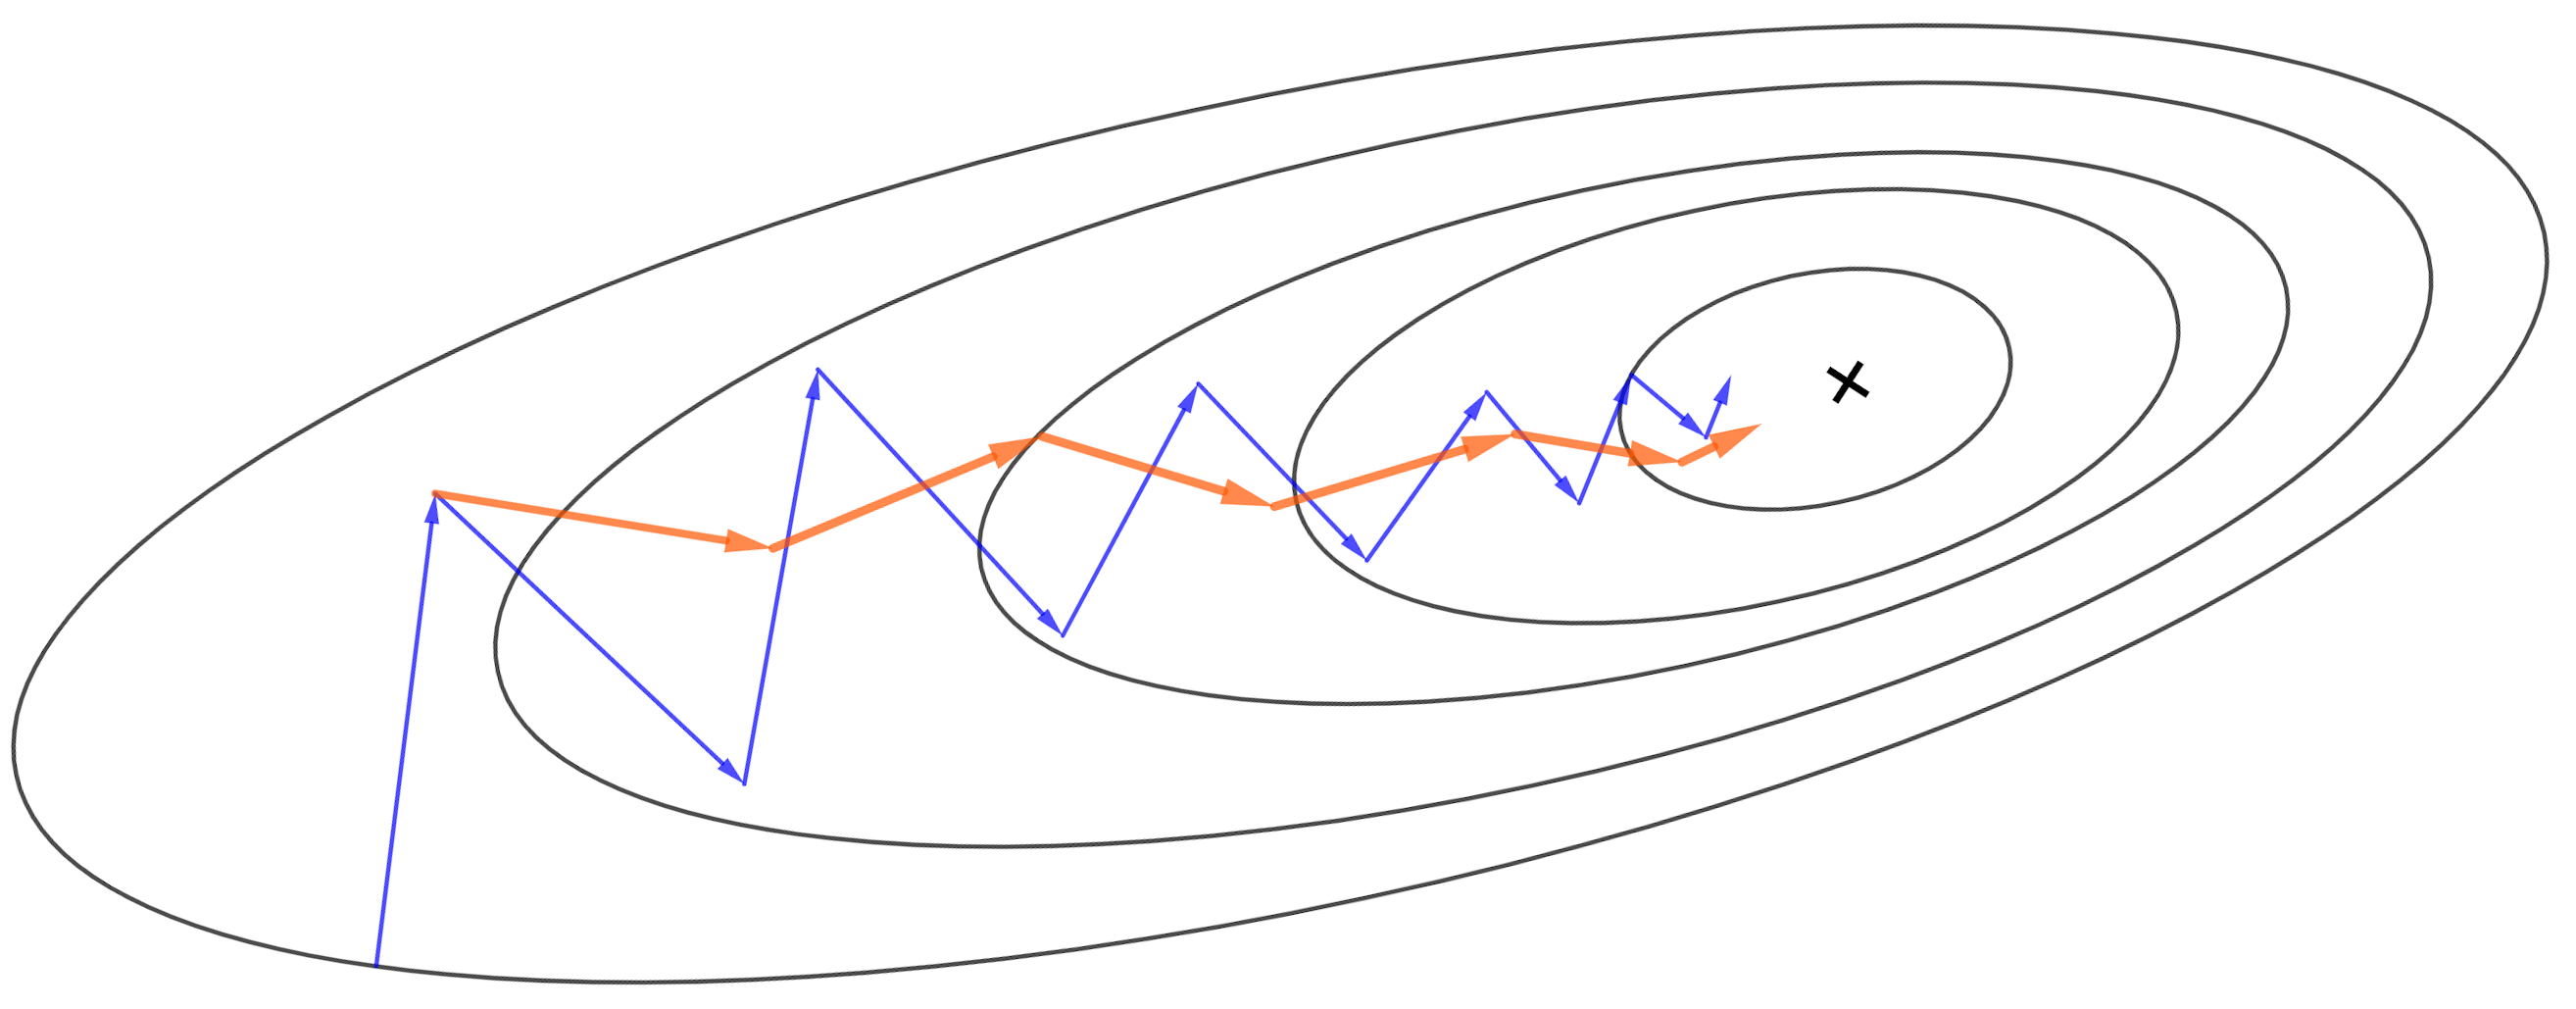
\includegraphics[width=\linewidth]{imgs_tomas/momentum.png}
%     \caption{Gradient Descent with Momentum}
%     \label{fig:momentum}
% \end{figure}

% \begin{algorithm}[ht]
% \caption{Structure Optimization}
% \label{alg:strucreal_gd}
% \begin{algorithmic}[1]
% \State Initialize $\bm{V}$
% \State Random sample of model parameters $(\phi, \psi)$
%     \Repeat
%         \State Forward pass through the model $\mathcal{G}((\phi, \psi))$
%         \State Calculate Loss
%         \State Backward pass - Calculate Gradients ($\nabla (\phi, \psi)$)
%         \State Normalize gradients
%         \State Update $\bm{V}$: $\bm{V} = \mu \bm{V} - \alpha \nabla (\phi, \psi)$
%         \State Update model parameters: $(\phi, \psi) = (\phi, \psi) + \bm{V}$
%     \Until{i = iterations}
% \end{algorithmic}
% \end{algorithm}

% In the first step we initialized a vector $\bm{V}$ which we used for implementing momentum. This is a simple idea the reuses gradient from previous iteration, where we no longer move in the direction of the steepest descent, but the direction is altered (dependent on the momentum parameter $\mu$) by adding the vector pointing in the direction of the last gradient. The principle of momentum is visualized on Figure \ref{fig:momentum}.

% The second step refers to sampling of the torsion angles from the angle distributions. We fitted a von-Misses distribution to the histograms. Von Mises distribution is a continouous distribution defined on a circle in range $[-\pi, \pi)$ with a bell like shape. Formally its probability density function is 
% $$\mathds{P} = \frac{e^{\kappa cos(x - \mu)}}{2\pi I_0(\kappa)}$$ 
% where $I_0(\kappa) = \sum_{i=0}^\infty \frac{\kappa^{2i}}{2^{2i}(i!)^2}$ is a modified Bessel Function with order zero. 
% The $\kappa$ parameter is called concentration ($\sim 1/\sigma^2$) and describes the dispersion and $\mu$ is the mean direction of the distribution \cite{vonmises}. 

% In the next step the algorithm enters a cycle which ends after specified number iterations. In the first step of each iteration the model of protein geometry is created from current torsion angles ($(\phi, \psi)$), which are the parameters of the model, and the coordinates of backbone + C$_\beta$ atoms are computed. Finally a distance matrix is computed between all C$_\beta$ atoms of all residues (C$_\alpha$ for glycine).

% We used the distance distributions predicted by the neural network to define a loss function:

% \begin{equation}
%      V_{dist}(\mathcal{G}((\phi, \psi))) = -\sum_{i, j, i \neq j} log[\mathds{P} (d_{ij} | S, MSA(S))]
%      \label{eq:dist_pot}
% \end{equation}

% which is a simple negative log-likelihood function. In order to calculate the loss at any inter-residue distance, we approximated the distance histograms with a normal distribution (scaled, so that its max probability is the same as for the particular distogram).

% The sixth step of the algorithm refers to a computation of the gradients, which thankfully is done automatically by pytorch by calling the \texttt{.backward} method. In order to avoid exploding gradients, we divided the gradients by their standard deviation before updating the parameters. This ensured that the gradients were roughly on the same scale throughout the algorithm interations, while preserving their orientations. In the 8th and 9th step the parameters are updated with the possibility of reusing previous gradients, by setting the momentum parameter $\mu > 0$.

\section{Evaluation Metrics}

In order to assess the performance of different models and most importantly, evaluate the closeness of the predictions to the reality a good metric is neccessary. The metrics used in protein folding protocols are usually divide into two classes: alignment free and alignment dependent. As the name of the first category suggests, these metrics do not require for the two structures to be aligned while the latter ones does. The advantage of the alignment free metrics is that they are faster to use, however the alignment requiring metrics provide more information. 

We will first describe an alignment free metric we used for comparing and choosing between our models (DlDDT) and then the TM-Score metric, already mentioned in the introduction.

\subsection{(D)lDDT - (Distogram) local Distance Difference Test}

The lDDT metric evaluates regions of distance matrices capturing local folding patterns. This means that only residues that are closer in reality than some threshold (usually $D_{ij} < 15$\AA) are compared. It is less affected by outliers than RMSD (Root Mean Squared Deviation) and correlates well with the global similarity measures.

The algorithm counts the number of inter-residue distances that are closer to the reality than another imposed threshold - it cycles through 4 different ones: $t \in \{0.5, 1, 2, 4\}$\AA \cite{lddt}.

The formula for comparing real distance matrix ($D$) and predicted one ($d$) for a domain of length $L$:

$$IDDT = \frac{100}{4} \sum_{t \in \{0.5, 1, 2, 4\}} \frac
{\sum_{i = 1}^L \sum_{j, |i - j| > 1, D_{ij} < 15} \mathds{1}(|D_{ij} - d_{ij}| < t)}
{\sum_{i = 1}^L \sum_{j, |i - j| > 1, D_{ij} < 15} 1} $$

However, since our models are essentialy classifiers and we predict a distribution of distances for each $D_{ij}$, Alphafold proposed a modified version of this metric. Instead of the indicator function in numerator it calculates probabilities of bins around the real distance that are closer to it than the treshold $t$. Formally:

\begin{equation}
DlDDT = \frac{100}{4} \sum_{t \in \{0.5, 1, 2, 4\}} \frac
{\sum_{i = 1}^L \sum_{j, |i - j| > 1, D_{ij} < 15} \mathds{P}(|D_{ij} - d_{ij}| < t~|~ \mathcal{S}, MSA)}
{\sum_{i = 1}^L \sum_{j, |i - j| > 1, D_{ij} < 15} 1}
    \label{eq:dlddt}
\end{equation}

\subsection{TM-score}

The Template Modelling score assesses the similarity between two three dimensional structures. As opposed to a simple RMSD metric, TM score is less inflated by outliers and favors folds with better aligned regions. TM-score also takes into account the length of the aligned region, which proved to be an important idea. The calculation requires structural alignment of the predicted and template structure\cite{tmscore}. The calculation and alignment of the structure was performed by the freely available TM-align package \cite{tmalign}.

% \begin{equation}
%     TMscore = Max \left[ \frac{1}{L_N} \sum_{i = 1}^{L_T} \frac{1}{1 + (\frac{d_i}{d_0})^2)} \right]
%     \label{eq:tmscore}    
% \end{equation}

